\documentclass[11pt]{article}
%\usepackage{authblk}
\usepackage{fullpage} % sets margins a bit smaller

% ##### Bibliography options
\usepackage{natbib}
\bibpunct{(}{)}{;}{a}{,}{,}

\usepackage{amsmath, amssymb, amsthm}
\usepackage[linesnumbered, ruled, vlined]{algorithm2e}
%\usepackage{algorithm} % delete these later, convert to algorithm2e
\usepackage{algorithmic} % delete these later, convert to algorithm2e
\usepackage[shortlabels]{enumitem}
\usepackage{xcolor}
\usepackage{booktabs}
\usepackage{multirow}
\usepackage{setspace}
\usepackage{caption}
\usepackage{graphicx}
\graphicspath{ {convg_diag_figures/} }
\usepackage{float}
\usepackage[pdftex,colorlinks=true,linkcolor=blue,citecolor=blue,urlcolor=blue,bookmarks=false,pdfpagemode=None]{hyperref}
\allowdisplaybreaks
\usepackage{subfig}

\SetKwInOut{Require}{Require}
\SetKwInOut{Input}{Input}\SetKwInOut{Output}{Output}
\newtheorem{definition}{Definition}[section]
\newtheorem{theorem}{Theorem}[section]
\newtheorem{lemma}[theorem]{Lemma}
\newtheorem{proposition}[theorem]{Proposition}
\newtheorem{assumption}[theorem]{Assumption}
\newtheorem{remark}[theorem]{Remark}
\newtheorem{corollary}[theorem]{Corollary}

\newcommand{\todo}[1]{\textcolor{red}{xx TODO: #1 xx}}
\newcommand{\comment}[1]{\textcolor{red}{[{ #1 }] } }

\newcommand{\Ex}[1]{\mathbb{E}[ #1 ]}
\newcommand{\EX}[1]{\mathbb{E}\left[ #1 \right]}
\newcommand{\R}{\mathbb{R}}
\usepackage[numbers]{natbib}
\usepackage[T1]{fontenc}
\usepackage{bm,amsmath,amsthm,amssymb,multicol,algorithmic,algorithm,enumitem}
\usepackage{wrapfig,lipsum}
\usepackage[textwidth=1cm,textsize=footnotesize]{todonotes}
\usepackage{caption}
% ready for submission
\usepackage{neurips_2020}
\usepackage{thm-restate}
\usepackage{comment}
\usepackage[colorlinks=true,
linkcolor=red,
urlcolor=blue,
citecolor=blue]{hyperref}
\usepackage{hyperref}
\usepackage{cleveref}
\usepackage{subfigure}
\usepackage{booktabs}
\setlength{\parskip}{.2cm}

 \makeatletter
\renewenvironment{proof}[1][\proofname]{%
   \par\pushQED{\qed}\normalfont%
   \topsep6\p@\@plus6\p@\relax
   \trivlist\item[\hskip\labelsep\bfseries#1]%
   \ignorespaces
}{%
   \popQED\endtrivlist\@endpefalse
}
\makeatother

%%%%%%%%%%% Stuffs for Tikz %%%%%%%%%%%%%%%%%%
\usepackage{pgfplots}
\usepackage{xargs}
\usepackage{stmaryrd}
\usetikzlibrary{arrows,shapes,calc,tikzmark,backgrounds,matrix,decorations.markings}
\usepgfplotslibrary{fillbetween}

\pgfplotsset{compat=1.3}

\usepackage{relsize}
\tikzset{fontscale/.style = {font=\relsize{#1}}
    }

%%%%%%%%%%%%%%%%%%%%%%%%%%%%%%%%%%%%%


\usepackage{shortcuts_OPT}

\makeatletter
\DeclareRobustCommand*\cal{\@fontswitch\relax\mathcal}
\makeatother

\begin{document}
\title{\vspace{-0.1in}Convergent Adaptive Gradient Methods in Decentralized Optimization\vspace{-0.15in}}
%\author{}
\date{\today}

\maketitle


\begin{abstract}\vspace{-0.1in}
Adaptive gradient methods including Adam, AdaGrad, and their variants are proven to be very successful for training machine learning models such as neural nets in the past a few years. At the same time, distributed optimization is becoming increasingly popular, partly due to its success in training neural nets.  With the growth of computing power and the need for using machine learning models on mobile devices, the communication cost of distributed training algorithms becomes unignorable. In response to this, more and more attention is shifted from the traditional parameter server training paradigm to decentralized training paradigms, which usually require lower communication costs. In this paper, we try to rigorously incorporate adaptive gradient methods into decentralized training, coming up with convergent decentralized adaptive gradient methods. Specifically, we propose an algorithmic framework that can convert existing adaptive gradient methods to their decentralized counterparts. In addition, we rigorously analyze the convergence behavior of the proposed algorithmic framework and show that if an adaptive gradient method satisfy some specific conditions, its converted counterpart is also convergent. Finally, using the framework, we proposed the first convergent decentralized adaptive gradient method.
\end{abstract}



\section{Introduction}
%\vspace{-0.1in}

Distributed training of machine learning models is drawing increasing attention in the past few years due to its practical benefits and necessities. Due to the evolution of computing capabilities of CPUs and GPUs, computation time in distributed training is gradually dominated by the communication time in many circumstances \citep{chilimbi2014project, mcmahan2016communication}. In response to this fact, a large amount of recent works has been focusing on reducing communication cost for distributed training \citep{alistarh2017qsgd,lin2017deep,wangni2018gradient,stich2018sparsified,wang2018atomo,tang2019doublesqueeze}. 
In the traditional parameter server setting where a parameter server is employed to manage communication in the whole network, many effective communication reductions have been proposed based on gradient compression and quantization. Despite these communication reduction techniques, the amount of data flow of the parameter server usually scales linearly with the number of workers.  Due to this limitation, there is a rising interest in the research community in the decentralized training paradigm \citep{duchi2011dual}, where the parameter server is removed and every node only communicates with its neighbors. It has been shown in \citet{lian2017can}  that decentralized training algorithms can outperform parameter server-based algorithms when the training bottleneck is the communication cost. The decentralized training paradigm is also preferred when a parameter server is not available. 


In parallel to distributed training, another effective way to accelerate training is by using adaptive gradient methods like AdaGrad \citep{duchi2011adaptive}, Adam \citep{kingma2014adam} and AMSGrad \citep{reddi2019convergence}. Their practical benefits are proven by their popularity in training neural nets, featured by faster convergence and ease of parameter tuning compared with SGD.

Despite a large amount of literature in distributed optimization, there have been few works seriously considering bringing adaptive gradient methods into distributed training, largely due to the lack of understanding in convergence behavior of adaptive gradient methods. 
 

In this paper, we investigate the possibility of using adaptive gradient methods in the decentralized training paradigm. 
Designing adaptive methods in such settings is highly non-trivial due to the already complicated update rules and the interaction between the effect of using adaptive learning rates and decentralized communication protocols.


The key result of this work is  a general technique that can convert an adaptive gradient method from a centralized method to a decentralized method. More importantly,
we provide a theoretical verification interface for analyzing the behavior of decentralized adaptive gradient methods converted by our technique.

By using our proposed technique, we also present a new decentralized optimization algorithm, called decentralized AMSGrad, converted by our technique from AMSGrad. Build on our proposed framework for analyzing the type of algorithms, we can characterize the convergence rate of decentralized AMSGrad, which is the first convergent decentralized adaptive gradient method.

 
  A novel technique in our framework is a mechanism to enforce a consensus on adaptive learning rates at different nodes. We show the importance of consensus on adaptive learning rates by proving a divergent problem instance for a recently proposed decentralized adaptive gradient method DADAM, which lacks consensus mechanisms on adaptive learning rates.

 
 \textbf{Notations}: $x_{t,i}$ denotes variable $x$ at node $i$ and iteration $t$. $\|\cdot \|_{abs}$ denotes the entry-wise $L_1$ norm of a matrix, i.e. $\|A\|_{abs}= \sum_{i,j} A_{i,j}$. For the ease of presentation, here we also introduce some notations that will be used later in the paper. 
\begin{multicols}{2}
 \begin{itemize}
 	\item $G_t = [g_{t,1}, g_{t,2}, ..., g_{t,N}]$

 	\item $M_t = [m_{t,1}, m_{t,2}, ..., m_{t,N}]$
 	
 	\item $X_t = [x_{t,1}, x_{t,2}, ..., x_{t,N}]$
 	
 	\item $\overline {\nabla f}(X_t) = \frac{1}{N}\sum_{i=1}^N \nabla f_i(x_{t,i})$
 	
 	\item $U_t = [u_{t,1}, u_{t,2}, ..., u_{t,N}]$
 	
 \item $ \tilde U_t = [ \tilde u_{t,1}, \tilde u_{t,2}, ...,  \tilde u_{t,N}]$
 \end{itemize}
\columnbreak
\begin{itemize}
	\item $ V_t = [ v_{t,1},  v_{t,2}, ...,  v_{t,N}]$
	
	\item $\hat V_t = [\hat v_{t,1}, \hat v_{t,2}, ..., \hat v_{t,N}]$
	
	\item $\overline X_t = \frac{1}{N}\sum_{i=1}^N x_{t,i} $
	
	\item $\overline U_t = \frac{1}{N}\sum_{i=1}^N u_{t,i} $
	
	\item $\overline {\tilde U_t} = \frac{1}{N}\sum_{i=1}^N  \tilde u_{t,i} $
\end{itemize}
\end{multicols}
Also, we will introduce a $N \times N$ matrix $W$ later in the paper, we denote $\lambda_i$ to be its $i$th largest eigenvalue and define $\lambda \triangleq \max (|\lambda_2|,|\lambda_N|)$.

 \vspace{-0.1in}
\section{Related work}
 \vspace{-0.1in}
\textbf{Decentralized optimization:} Decentralized optimization has a long history, traditional decentralized optimization methods include well-know algorithms such as ADMM \citep{boyd2011distributed}, dual averaging 
\citep{duchi2011dual}, distributed subgradient descent \citep{nedic2009distributed}. More recent algorithms include Extra \citep{shi2015extra}, Next \citep{di2016next} and Prox-PDA \citep{hong2017prox}.  While these algorithms were commonly used in applications other than deep learning, recent algorithmic advances in the machine learning community have shown that decentralized optimization can be useful for training neural nets. \citet{lian2017can} showed that a stochastic version of decentralized subgradient descent can outperform parameter server-based algorithms when the communication cost is high. \citep{tang2018d} proposed $D^2$ that improves the convergence rate over stochastic subgradient descent. \citep{assran2018stochastic} proposed the Stochastic Gradient Push that is more robust to network failures for training neural nets. The study of decentralized training in the machine learning community is only at its initial stage. No one has seriously considered designing adaptive gradient methods in the setting of decentralized training until the recent work \citet{nazari2019dadam}, a decentralized version of AMSGrad \citep{reddi2019convergence} is proposed in \citet{nazari2019dadam} and it is proven to satisfy some non-standard regret. 


\textbf{Adaptive gradient methods:}  Adaptive gradient methods are popularized in recent years due to their superior performance in training neural nets. The type of methods usually refers to AdaGrad \citep{duchi2011adaptive}, Adam \citep{kingma2014adam}, and their variants.  Key features of such methods include the use of momentum and adaptive learning rates (which means the learning rate is changing during optimization and the learning rates on different coordinates might be different). The most adaptive gradient is Adam, which is believed to converge until the recent work \citet{reddi2019convergence} pointed out an error in the convergence analysis of Adam. Since then, many research efforts in the community are investigated into analyzing the convergence behavior of adaptive gradient methods. \citet{ward2018adagrad, li2018convergence} analyzed convergence of a variant of AdaGrad without coordinate-wise learning rates. \citet{chen2018convergence} analyzed the convergence behavior of a broad class of algorithms including AMSGrad \citep{reddi2019convergence} and AdaGrad. \citet{zou2018convergence} provided a unified convergence analysis for AdaGrad with momentum.    A few recent adaptive gradient methods can be found in \citet{agarwal2018case,luo2019adaptive,zaheer2018adaptive}.  


vspace{-0.1in}
\section{Decentralized training and divergence of DADAM}
\vspace{-0.1in}

\subsection{Decentralized optimization }
In distributed optimization (with $N$ nodes), we aim at solving the following problem
\begin{align}
\min_{x} \frac{1}{N}\sum_{i=1}^N f_i(x)
\end{align}
where $f_i$ is only accessible by the $i$th node. For neural net training, $f_i$ can be viewed as the average loss of data located at node $i$. 

Throughout the paper, we make the following assumptions for analyzing the convergence behavior of different algorithms.

\textbf{Assumptions}

A1: $f_i$'s are differentiable and the gradients is $L$-Lipschitz, i.e. $\|\nabla f_i(x) - \nabla f_i(y) \| \leq L\|x-y\|, \forall x,y$.

A2:  We assume at iteration $t$, node $i$ can access a stochastic gradient $g_{t,i}$. In addition,  the stochastic gradients have bounded $L_{\infty}$ norm and the gradients of $f_i$ are also bounded, i.e. $\|g_{t,i}\| \leq G_{\infty}$, $\|\nabla f_i(x)\|_{\infty} \leq G_{\infty}$. 

A3: The gradient estimators are unbiased and each coordinate have bounded variance, i.e. $\mathbb E [g_{t,i}] = \nabla f_i(x_{t,i}) $ and $\mathbb E [([g_{t,i} - f_i(x_{t,i})]_j)^2] \leq  \sigma^2, \forall t,i,j$ . 

The assumptions A1 and A3 are standard in distributed optimization. A2 is a little stronger than the traditional assumption that the estimator has bounded variance, it is commonly used in analyses for adaptive gradient methods \citep{chen2018convergence,ward2018adagrad}. One thing that should be noted is that the bounded gradient estimator assumption in A2 implies the bounded variance assumption in A3, we denote the variance bound and the estimator bound differently to avoid confusion when we use them for different purposes. 


In decentralized optimization, the nodes are connected as a graph and each node only communicates to its neighbors. In such cases, one usually construct a matrix $W$ for information sharing when designing algorithms. As can be expected, $W$ cannot be arbitrary, the key properties required for $W$ are listed in A4.

A4: Assumptions on matrix $W$.

 1). $\sum_{j=1}^N W_{i,j} = 1$,  $\sum_{i=1}^N W_{i,j} = 1$, $W_{i,j} \geq 0$. 
 
 2). Denote $\lambda_i$ to be $i$th largest eigenvalue of $W$, we have $\lambda_1 = 1$, $|\lambda_2| < 1$, $|\lambda_N| < 1 $.
 
 3). $W_{i,j} = 0 $ if node $i$ and node $j$ are not neighbors.
 
 Throughout this paper, we will assume A1-A4 hold. 





\subsection{Divergence of DADAM}

Recently, \citet{nazari2019dadam} initiated a trial to bring adaptive gradient methods into decentralized optimization, the resulting algorithm is DADAM, which is shown in Algorithm 1.
\begin{algorithm}[htbp]
	\caption{DADAM(with N nodes)}
	\label{alg: dadam}
	\begin{algorithmic}[1]
		\STATE {\bfseries Input:} learning rate $\alpha$, current point $X_t$, $u_{\frac{1}{2},i} = \hat v_{0,i} = \epsilon \mathbf{1}, \forall i$, $m_0=0$ mixing matrix $W$
		\FOR {$t = 1,2,..., T$}
		\STATE  $g_{t,i}  \leftarrow \nabla f_i(x_{t,i}) + \xi_{t,i}$
		\STATE $m_{t,i} = \beta_1 m_{t-1,i} + (1-\beta_1) g_{t,i}$ 
		\STATE $v_{t,i} = \beta_2 v_{t-1,i}+(1-\beta_2)g_{t,i}^2$
		\STATE $\hat v_{t,i} = \beta_3 \hat v_{t,i} + (1-\beta_3) \max(\hat v_{t-1,i},v_{t,i})$
		\STATE $x_{t+\frac{1}{2},i} = \sum_{j=1}^N W_{ij}x_{t,j}$
		\STATE $x_{t+1,i} = x_{t+\frac{1}{2},i} - \alpha \frac{m_{t,i}}{\sqrt{\hat v_{t,i}}}$
		\ENDFOR
	\end{algorithmic}
\end{algorithm}

DADAM is essentially a decentralized version of AMSGrad and the key modification is the use of a consensus step on optimization variable $x$ to transmit information across the network, encouraging convergence. The matrix $W$ is a doubly stochastic matrix (which satisfies A4) for achieving  average consensus of $x$. Introducing such a mixing matrix is a standard approach for decentralizing an algorithm, such as distributed gradient descent \citep{nedic2009distributed, yuan2016convergence}. It is proven in \citet{nazari2019dadam} that DADAM admits a non-standard regret bound in the online setting, however, whether the algorithm can converge to stationary points in standard offline settings such training neural nets is still unknown.


In the following, we show the DADAM may fail to converge in offline nonconvex optimization settings.
\begin{restatable}{theo}{dadam_diverge}\label{thm: dadam_diverge}
	There exist a problem satisfying $A1 -A4$ where DADAM fail to converge.   
\end{restatable} 
\textbf{Proof}: 
Consider  a 1 dimensional optimization problem distributed onto two nodes
{\small
\begin{align}
\min_{x} \frac{1}{2 }\sum_{i=1} ^2 f_i(x)
\end{align}
}%
where $ f_i(x) =  \frac{1}{2} (x - a_i)^2$ and $a_1 = 0$, $a_2 = 1$.


The network contains only two nodes and the matrix $W
$ satisfy $W_{ij} = \frac{1}{2}, \forall i,j$. 

We consider running DADAM with $\beta_1 = \beta_2 = \beta_3 = 0$ and $\epsilon = 0.6$ for simplicity.   Suppose we initialize DADAM at $x_{1,i} = 0, \forall i$ and use learning rate $\alpha = 0.001$.  We have at $x_{1,i} = 0$, $\nabla f_1(x_{1,1}) = 0$,  $\nabla f_2(x_{1,2}) = 1$, this will lead to $\hat v_{1,1} = 0.6$ and $\hat v_{1,2} = 1$. Thus, from step 1, we will have $\hat v_{1,2} \geq 1$. In addition, it s easy proved that with the stepsize selection, we always have $\hat v_{1,1} < 1 $, in fact, it will not even reach 0.6.
 Thus, in the later iterations, the gradient of losses on node 1 and 2 will be scaled  differently.  This scaling is equivalent running gradient descent on a objective where the losses of the two nodes are scaled by different factors.  In such a case, the algorithm will converge to a stationary point of a weighted average of the loss on node $1$. Since the  weight of the losses on the two nodes are different and the problem is a quadratic problem with only one minimizer and the unbalanced weights on the two functions yields a different minimizer, the algorithm will not converge to the unique stationary point of the original loss (which is $x=0.5$). \hfill $\square$

Theorem \ref{thm: dadam_diverge} says that though DADAM is proven to satisfy some regret bounds \citep{nazari2019dadam}, it can fail to converge to stationary points in the nonconvex offline setting, which a common setting for training neural nets. We conjecture that this inconsistency is due to the definition of the regret in \citet{nazari2019dadam}. In the next section, we will design decentralized adaptive gradient methods that are guaranteed to converge to stationary points. 





\vspace{-0.1in}
\section{Convergent decentralized adaptive gradient methods}
\vspace{-0.1in}

In this section, we will discuss difficulties of designing adaptive gradient methods in decentralized optimization and introduce an algorithmic framework that will convert existing convergent adaptive gradient methods to their decentralized counterparts. By using the framework, we proposed the first convergent decentralized adaptive gradient method, converted from AMSGrad.

\subsection{Importance and difficulties of consensus on adaptive learning rates}


The divergent example in the previous section implies that we should synchronize the adaptive learning rates on different nodes. This can be easy to achieve in the parameter server setting where all the nodes are sending their gradients to a parameter server at each iteration. The parameter server can use the received gradients to maintain a sequence of synchronized adaptive learning rates when updating the parameters. However, in the situation of decentralized training, every node can only communication with its neighbors and a parameter server does not exist.   
Since every node can only communicate with its neighbors, the information for updating the adaptive learning rates can be only shared locally instead of broadcasted over the whole network, this make it impossible to obtain an synchronized updated adaptive learning rate in a single iteration using all the information in the network. 

One way to solve this problem is to design communication  protocols to give each node access to the same aggregated gradients over the whole network at least periodically if not at every iteration, so that the nodes can update their individual adaptive learning rates based on the same information to generate a synchronized sequence of adaptive learning rates. However, such a solution will introduce a significant amount of extra communication cost since it involves broadcasting over the network. Also, this is more of a system level solution instead of a algorithmic level solution. 

Another way to solve this problem is by letting the  sequences of adaptive learning rates on different nodes consent gradually, as the number of iteration grows. Intuitively, if the adaptive learning rates can consent fast enough, the difference among the adaptive learning rates on different nodes will not affect the convergence of the algorithm.  The benefit of such an approach is that we do not need to introduce too much extra communication cost and as we will show later, it will produce an framework that automatically convert existing adaptive gradient methods to their decentralized counterparts. Yet, the benefits do not come for free.  One need to design a way to ensure consensus of adaptive learning rates and this procedure should have a relatively low cost and be easy to implement. More importantly, such a design will further complicates the already convoluted convergence analysis of adaptive gradient methods. 

In the next section, we will introduce our designed algorithmic framework based on this approach and its theoretical guarantee.
\subsection{On decentralized adaptive gradient methods}
 As mentioned before, we need to choose a method to implement consensus of adaptive learning rates and there are many ways to do this. While each node can have different $\hat v_{t,i}$ in DADAM, one can keep track of the min/max/average of these adaptive learning rates and use the tracked quantity to update the adaptive learning rates. Also one can predefined some convergent lower and upper bounds to gradually synchronize the adaptive learning rates on different nodes like what the authors did for AdaBound \citep{luo2019adaptive}.  We choose to use average consensus on $\hat v_{t,i}$ because in adaptive gradient methods such as AdaGrad and Adam, $\hat v_{t,i}$ approximate the second moment of gradient estimator, the average of estimations of second moments from different nodes is an estimation of second moment on the whole network.  Also, this design will not introduce any extra tunable parameters that will complicates the parameter tuning process. 
 
 
 
\begin{algorithm}[hbtp]
	\caption{decentralized adaptive gradient method (with N nodes)}
	\label{alg: dadaptive}
	\begin{algorithmic}[1]
		\STATE {\bfseries Input:} learning rate $\alpha$, initial point $x_{1,i} = x_{init}, u_{\frac{1}{2},i} = \hat v_{0,i}, m_{0,i}=0, \forall i$, mixing matrix $W$
		\FOR{$t=1,2,...,T$}
		\STATE  $g_{t,i}  \leftarrow \nabla f_i(x_{t,i}) + \xi_{t,i}$
		\STATE $m_{t,i} = \beta_1 m_{t-1,i} + (1-\beta_1) g_{t,i}$ 
		\STATE $\hat v_{t,i} = r_t(g_{1,i},...,g_{t-1,i})$
		\STATE $x_{t+\frac{1}{2},i} = \sum_{j=1}^N W_{ij}x_{t,j}$
	    \STATE $\tilde u_{t,i} = \sum_{j=1}^N W_{ij} \tilde u_{t-\frac{1}{2},j}$
	    \STATE $u_{t,i} = \max(\tilde u_{t,i}, \epsilon)$
		\STATE $x_{t+1,i} = x_{t+\frac{1}{2},i} - \alpha \frac{m_{t,i}}{\sqrt{u_{t,i}}}$
		\STATE $\tilde u_{t+\frac{1}{2},i} = \tilde u_{t,i} - \hat v_{t-1,i} + \hat v_{t,i}$
		\ENDFOR
	\end{algorithmic}
\end{algorithm}


Theorem \ref{thm: dagm_converge} presents the convergence guarantee of Algorithm \ref{alg: dadaptive}.
\begin{restatable}{theo}{dagm_converge}\label{thm: dagm_converge}
	Assume  $\|g_{t,i}\|_{\infty} \leq G_{\infty}$,  $\|\nabla f_i(x)\|_{\infty} \leq G_{\infty} $ and set $\alpha = 1/
	\sqrt{Td}$. When $\alpha  \leq \frac{\epsilon^{0.5}}{16L} $, 
	  Algorithm 2 yields the following regret bound
	{\small 
	\begin{align}\label{eq: thm1}
	 \frac{1}{T}\sum_{t=1}^T  \mathbb E \left [\left\|\frac{\nabla f( \overline X_{t})}{\overline U_{t}^{1/4}}\right\|^2  \right] 
	\leq  & C_1 \frac{\sqrt{d}}{\sqrt{T}} \left(\mathbb E  [f( Z_{1})]  - \min_{z} f(z)  + \frac{\sigma^2}{N}\right)  +  \frac{ C_2 }{T}    + \frac{C_3}{T^{1.5}d^{0.5}}  \nonumber \\ 
	&+ \left(  \frac{C_4}{T N^{0.5} }  + \frac{C_5}{T^{1.5}d^{0.5} N^{0.5}}   \right) \mathbb E \left[ \sum_{t=1}^{T}   \|    (- \hat V_{t-2} + \hat V_{t-1} ) \|_{abs} \right]  
	\end{align}
	}%
	where $\| \cdot\|_{abs}$  denotes the entry-wise $L_1$ norm of a matrix (i.e $\| A\|_{abs} = \sum_{i,j}{|A_{ij}|}$) and $C_1, C_2 ,C_3, C_4, C_5$ are defined as 
	{\small
	\begin{align}
	C_1 = & \max (4, 4{L/\epsilon}) \nonumber \\
	C_2 = & 6 \left(\left( \frac{\beta_1}{1-\beta_1}\right)^2 + \left (\frac{1}{1-\lambda} \right)^2 \right)L  \frac{G_{\infty}^2 }{\epsilon^{1.5}}   \nonumber \\
	C_3 = & 16L^2 \left ( \frac{1}{1-\lambda}\right) \frac{G_{\infty}^2}{\epsilon^2} \nonumber \\
	C_4 = &  \frac{2}{ \epsilon^{1.5}}   \frac{1}{1-\lambda}  \left(     \lambda + \frac{\beta_1}{1-\beta_1}    \right){G_{\infty}^2} \nonumber \\
	C_5 = &  \frac{2}{ \epsilon^{2}}   \frac{1}{1-\lambda}   L   \left ( \frac{\beta_1}{1-\beta_1} \right)^2 {G_{\infty}^2}  + \frac{4}{ \epsilon^{2}}   \frac{\lambda}{1-\lambda}   L    {G_{\infty}^2}   
	\end{align}
	}%
	which are constants independent of $d$, $T$ and $N$.
\end{restatable}
\textbf{Proof:} The proof can be found in Appendix \ref{app: proof_thm_adm}. 
%The proof sketch can be found in Section \ref{sec: proof_sketch} and the complete proof can be found in Appendix \ref{app: proof_thm_adm}. 

\textbf{Remark:} From the theorem, it can be seen that if $\mathbb E \left[ \sum_{t=1}^{T}   \|    (- \hat V_{t-2} + \hat V_{t-1} ) \|_{abs} \right]  = o(T)$ and $\bar U_t$ is upper bounded, the algorithm is guaranteed to converge to stationary points. Intuitively, this says that if the adaptive learning rates on different nodes do not change too fast, the algorithm can converge. This is intuitively true as in \citet{chen2018convergence}, it is shown that if such a condition is violated, an algorithm can diverge. Furthermore, the theorem shows the benefit of using more nodes. As $N$ becomes larger, the term $\sigma^2/N$ will be small, this is also justified by intuition that with the growth of $N$, the training process tends to be more stable. 





In the following, we will present a notable special case of our algorithmic framework, decentralized AMSGrad, which is a decentralized variant of AMSGrad in our framework.

\begin{algorithm}[htbp]
	\caption{decentralized AMSGrad (with N nodes)}
	\label{alg: damsgrad}
	\begin{algorithmic}[1]
		\STATE {\bfseries Input:} learning rate $\alpha$, initial point $x_{1,i} = x_{init}, u_{\frac{1}{2},i} = \hat v_{0,i} = \epsilon \mathbf 1\ (\text{with } \epsilon \geq 0), m_{0,i}=0, \forall i$, mixing matrix $W$ 
		\FOR{$t = 1,2,...,T$}
		\STATE  $g_{t,i}  \leftarrow \nabla f_i(x_{t,i}) + \xi_{t,i}$
		\STATE $m_{t,i} = \beta_1 m_{t-1,i} + (1-\beta_1) g_{t,i}$ 
		\STATE $ v_{t,i} = \beta_2 v_{t-1,i} + (1-\beta_2) g_{t,i}^2 $
		\STATE $\hat v_{t,i} = \max (\hat v_{t-1,i}, v_{t,i} )$
		\STATE $x_{t+\frac{1}{2},i} = \sum_{j=1}^N W_{ij}x_{t,j}$
		\STATE $\tilde u_{t,i} = \sum_{j=1}^N W_{ij}\tilde u_{t-\frac{1}{2},j}$
	    \STATE $u_{t,i} = \max(\tilde u_{t,i}, \epsilon)$
		\STATE $x_{t+1,i} = x_{t+\frac{1}{2},i} - \alpha \frac{m_{t,i}}{\sqrt{u_{t,i}}}$
		\STATE $\tilde u_{t+\frac{1}{2},i} = \tilde u_{t,i} - \hat v_{t-1,i} + \hat v_{t,i}$
		\ENDFOR
	\end{algorithmic}
\end{algorithm}


Compared with DADAM, the above algorithm uses a dynamic average consensus mechanism to keep track of average of $\{\hat v_{t,i}\}_{i=1}^N$, stored as $\tilde u_{t,i}$ on $i$th node, and uses $u_{t,i} = \max(\tilde u_{t,i}, \epsilon)$ for updating the adaptive learning rate for $i$th node. As the number of iteration grows, even though $\hat v_{t,i}$ on different nodes can converge to different constants, all the $u_{t,i}$ will be converge to the same number $ \lim_{t \rightarrow \infty}\frac{1}{N}\sum_{i=1}^N\hat v_{t,i} $ if the limit exists. The use of this average consensus mechanism enables the consensus of adaptive learning rates on different nodes, which consequentially guarantees convergence to stationary points. The consensus of adaptive learning rates is the key difference between decentralized AMSGrad and DADAM and is the reason why decentralized AMSGrad is a convergent algorithm while DADAM is not. 




The following theorem presents the convergent guarantee of Algorithm \ref{alg: damsgrad}.


\begin{restatable}{theo}{dams_converge}\label{thm: dams_converge}
	Assume  $\|g_{t,i}\|_{\infty} \leq G_{\infty}$,  $\|\nabla f_i(x)\|_{\infty} \leq G_{\infty} $ 
	and set $\alpha = 1/
	\sqrt{Td}$. When $\alpha  \leq \frac{\epsilon^{0.5}}{16L} $, 
	  Algorithm \ref{alg: damsgrad} yields the following regret bound
	  {\small 
	  \begin{align}\label{eq: thm_ams}
	  & \frac{1}{T}\sum_{t=1}^T  \mathbb E \left [\left\|\frac{\nabla f( \overline X_{t})}{\overline U_{t}^{1/4}}\right\|^2  \right] 
	  \leq    C_1' \frac{\sqrt{d}}{\sqrt{T}} \left(\mathbb E  [f( Z_{1})]  - \min_{z} f(z)]  + \frac{\sigma^2}{N}\right)  +  \frac{ C_2'}{T}    +   \frac{d}{T }\sqrt{N} C_4' + \frac{\sqrt{d}}{T^{1.5} } \sqrt{N} C_5'
	  \end{align}
	  }%
	where 
	\begin{align}
	&C_1' = C_1,\
	C_2' = C_2,\
	 C_3' = C_3, \nonumber \\
	  &C_4' = C_4G_{\infty}^2,\
	 C_5' = C_5 G_{\infty}^2 
	\end{align}
	and $C_1,C_2, C_3, C_4, C_5$ are constants independent of $d$, $T$ and $N$ defined in Theorem \ref{thm: dagm_converge}.
\end{restatable}
\textbf{Proof:} See Appendix \ref{app: proof_ams}

\textbf{Remark:} The above theorem says that Algorithm \ref{alg: damsgrad} converges with a rate of $O(\sqrt{d}/\sqrt{T})$ when $T$ is large, which is the best known convergence rate under the given assumptions. Note that in some literature, SGD admits a convergence rate of $O(1/\sqrt{T})$ without any dimension dependency, such an improved convergence rate is under the assumption that the gradient estimator have bounded $L_2$ norm, which can hide a dimension dependency of $\sqrt{d}$ in the final convergence rate. One can 

In the next section, we will present the proof sketch of Theorem \ref{thm: dagm_converge} since the whole proof is complicated and the convergence analysis is one of our main contributions.


% \vspace{-0.1in}
% \section{Proof Sketch of Theorem \ref{thm: dagm_converge}}\label{sec: proof_sketch}
% \vspace{-0.1in}

% In this section, we will present the proof sketch for convergence analysis of Algorithm \ref{alg: dadaptive} (proof sketch of Theorem \ref{thm: dagm_converge}). 


% To prove convergence of the algorithm, we need to first define an auxiliary sequence of iterates
% {\small
% \begin{align}\label{eq: seq_z_sketch}
% Z_{t} = \overline X_t + \frac{\beta_1}{1-\beta_1} (\overline X_t - \overline X_{t-1})
% \end{align}
% }%
% with $\overline X_{0} \triangleq \overline X_1$.

% Such an auxiliary sequence can help us deal with the bias brought by the momentum and simplifies the convergence analysis. Similar constructions are also used for analyzing SGD with momentum and centralized adaptive gradient methods \citep{yan2018unified, chen2018convergence}.

% One can then prove that the auxiliary sequence $Z_t$ follows the update rule
% {\small
% \begin{align}\label{eq: update_z_sketch}
% Z_{t+1} - Z_t = &\alpha \frac{\beta_1}{1-\beta_1}  \frac{1}{N} \sum_{i=1}^N m_{t-1	,i} \odot (\frac{1}{\sqrt{u_{t-1,i}}} - \frac{1}{\sqrt{u_{t,i}}}) - \alpha \frac{1}{N} \sum_{i=1}^N \frac{g_{t,i}}{\sqrt{u_{t,i}}}.
% \end{align}
% }%
% The above update rule is desired because momentum does not appear in the quantity $\frac{1}{N} \sum_{i=1}^N \frac{g_{t,i}}{\sqrt{u_{t,i}}}$ and this simplification is helpful because it is directly related to the current gradients instead of the exponential average of past gradients. 

% Then by smoothness, we have the basic inequality in nonconvex optimization
% {\small
% \begin{align}
% f( Z_{t+1}) \leq f( Z_{t}) + \langle \nabla f( Z_{t}),  Z_{t+1}-  Z_{t} \rangle + \frac{L}{2}\| Z_{t+1}-  Z_{t}\|^2 
% \end{align}}% 
% which will translate into
% {\small
% \begin{align}\label{eq: exp_lip_sketch}
% &\alpha  \mathbb E\left[\left \langle \nabla f( Z_{t}), \frac{1}{N} \sum_{i=1}^N \frac{\nabla f_i(x_{t,i})}{\sqrt{u_{t,i}}}  \right \rangle \right] \nonumber \\
% \leq & \mathbb E  [f( Z_{t})]  -  \mathbb E [f( Z_{t+1})] + \frac{L}{2} \mathbb E\left[\| Z_{t+1}-  Z_{t}\|^2 \right] + \alpha \frac{\beta_1}{1-\beta_1}  \mathbb E \left [\left \langle \nabla f( Z_{t}) , \frac{1}{N} \sum_{i=1}^N  \left(\frac{m_{t-1	,i}}{\sqrt{u_{t-1,i}}} - \frac{m_{t-1	,i}}{\sqrt{u_{t,i}}}\right) \right \rangle \right]
% \end{align}
% }%
% after taking expectation and rearranging.

% As in almost all convergence analyses, we will need to convert the LHS of the above inequality to the norm of gradients and upper bound all the quantities on the RHS to derive its convergence rate. We will do so now.

% We use following inequality to split out the norm of gradients from LHS of \eqref{eq: exp_lip_sketch}
% {\small
% \begin{align} \label{eq: split_1_sketch}
% &\left \langle \nabla f( Z_{t}), \frac{1}{N} \sum_{i=1}^N \frac{\nabla f_i( x_{t,i})}{\sqrt{\overline U_{t}}}  \right \rangle \nonumber \\
% \geq & \frac{1}{2} \left\|\frac{\nabla f( \overline X_{t})}{\overline U_{t}^{1/4}}\right\|^2   - \frac{3}{2} \left\|\frac{\nabla f( Z_{t}) -\nabla f( \overline X_{t})}{\overline U_{t}^{1/4}}\right\|^2- \frac{3}{2} \left\|  \frac{ \frac{1}{N}\sum_{i=1}^N \nabla f_i( x_{t,i}) -  \nabla f( \overline X_{t})}{\overline U_{t}^{1/4}}  \right\|^2
% \end{align}
% }%
% Then summing over $t$ from 1 to $T$ and do some simple algebraic manipulations, we can get 
% {\small
% \begin{align} \label{eq: exp_telescope_sketch}
% &\frac{1}{T}\sum_{t=1}^T  \mathbb E \left [\left\|\frac{\nabla f( \overline X_{t})}{\overline U_{t}^{1/4}}\right\|^2  \right] \nonumber \\
% \leq & \frac{2}{T\alpha} ( \mathbb E  [f( Z_{1})]  -  \mathbb E [f( Z_{T+1})]) + \frac{L}{T\alpha} \sum_{t=1}^T\mathbb E\left[\| Z_{t+1}-  Z_{t}\|^2 \right] \nonumber  \\
% &+ \frac{2}{T}\frac{\beta_1}{1-\beta_1} \underbrace{\sum_{t=1}^T   \mathbb E \left [\left \langle \nabla f( Z_{t}) , \frac{1}{N} \sum_{i=1}^N   (\frac{m_{t-1	,i}}{\sqrt{u_{t-1,i}}} - \frac{m_{t-1	,i}}{\sqrt{u_{t,i}}}) \right \rangle \right]}_{T_1} \nonumber \\
% & + \frac{2}{T} \underbrace{\sum_{t=1}^T \mathbb E \left [ \left \langle \nabla f( Z_{t}), \frac{1}{N} \sum_{i=1}^N \left( \frac{\nabla f_i( x_{t,i})}{\sqrt{\overline U_{t}}} -\frac{\nabla f_i( x_{t,i})}{\sqrt{u_{t,i}}}  \right)  \right \rangle \right] }_{T_2} \\
% & \begin{rcases}+ \frac{3}{T} \sum_{t=1}^T \mathbb E \left [ \left\|  \frac{ \frac{1}{N}\sum_{i=1}^N \nabla f_i( x_{t,i}) -  \nabla f( \overline X_{t})}{\overline U_{t}^{1/4}}  \right\|^2 \right] \nonumber \\
% + \frac{3}{T} \sum_{t=1}^T \mathbb E \left [ \left\|\frac{\nabla f( Z_{t}) -\nabla f( \overline X_{t})}{\overline U_{t}^{1/4}}\right\|^2 \right]
% \end{rcases} {T_3}.
% \end{align}
% }%

% Then we need to upper bound $T_1, T_2, T_3$ and the quadratic term of $Z_{t+1} - Z_t$. 

% We first bound $T_3$ since it is the most complicated term. By using smoothness again, it can be upper bound by quantities proportional to 
% {\small
% \begin{align}
% \sum_{t=1}^T\left\|  Z_{t} -  \overline X_{t}\right\|^2  \text{\ \ and\ \ }
% \sum_{t=1}^T\frac{1}{N}\sum_{i=1}^N\left\| {  x_{t,i} -   \overline X_{t}}  \right\|^2.
% \end{align}
% }%
% While the former quantity can be bounded as 
% \begin{align}
% \sum_{t=1}^T\left\|  Z_{t} -  \overline X_{t}\right\|^2  \leq T \left( \frac{\beta_1}{1-\beta_1}\right)^2 \alpha^2 d \frac{G_{\infty}^2}{\epsilon}
% \end{align}
% using update rule of $X_t$ and definition of $Z_t$, the later quantity requires a more complicated analysis which yields 
% {\small
% \begin{align} \label{eq: T_5_bound_sketch}
%  \sum_{t=1}^T \frac{1}{N}	\sum_{i=1}^N\left\| {  x_{t,i} -   \overline X_{t}}  \right\|^2   \leq T \alpha^2 \left (\frac{1}{1-\lambda} \right)^2 d G_{\infty}^2 \frac{1}{\epsilon}
% \end{align}
% }%
% where $\lambda = \max (|\lambda_2|,|\lambda_N|)$ and recall that $\lambda_i$ is $i$th largest eigenvalue of $W$.

% With the above inequalities, we can get an upper bound for $T_3$ proportional to $\alpha^2$, when $\alpha$ is small, this will be a small quantity (as will be evident later, the dominant quantity is in the order of $\alpha$).

% Now we need to look at $T_2$, after some derivation,  this term can be upper bounded by 
% {\small
% \begin{align}
% T_2 \leq & \frac{G_{\infty}^2}{N} \mathbb E \left[\sum_{t=1}^T \frac{1}{2\epsilon^{1.5}}  \| - \sum_{l=2}^N  \tilde U_t q_l q_l^T \|_{abs} \right] 
% \end{align}
% }%
% where $q_l$ is the eigenvector corresponding to $l$th largest eigenvalue of $W$ and   $\|\cdot\|_{abs}$ is the entry-wise $L_1$ norm of  matrices.

% In addition, after going through some further analysis, we can show that 
% {\small
% \begin{align}
% \sum_{t=1}^T  \| - \sum_{l=2}^N  \tilde U_t q_l q_l^T \|_{abs}  \leq {\sqrt{N}} \sum_{o=0}^{T-1} \frac{\lambda}{1-\lambda}     \|    (- \hat V_{o-1} + \hat V_{o} ) \|_{abs} 
% \end{align}
% }%
% which can finally show that  $T_2$ admits an upper bound proportional to $\sum_{o=0}^{T-1}  \|    (- \hat V_{o-1} + \hat V_{o} ) \|_{abs} $.

% As for $T_1$, using some similar techniques for bounding $T_2$, we can also upper bound it as a quantity proportional to $\sum_{o=0}^{T-1}  \|    (- \hat V_{o-1} + \hat V_{o} ) \|_{abs} $, which is
% {\small
% \begin{align}
% T_1 \leq G_{\infty}^2 \frac{1}{2\epsilon^{1.5}} \frac{1}{\sqrt{N}}   \mathbb E \left [  \frac{1}{1-\lambda}   \sum_{t=1}^T  \| ( - \hat V_{t-2} + \hat V_{t-1}) \|_{abs}   \right]
% \end{align}
% }%
% What remains is to upper bound $\sum_{t=1}^T \mathbb E\left[\| Z_{t+1}-  Z_{t}\|^2 \right]$ in \eqref{eq: exp_telescope_sketch}.  Upper bounding this term is another difficult task because we want to show the scaling of variance with respect to $N$ and the variance is hidden in the quantity.

% To bound this term, we first show that 
% {\small\begin{align}
% \| Z_{t+1}-  Z_{t}\|^2  
% \leq & 2 \alpha^2 \left ( \frac{\beta_1}{1-\beta_1} \right)^2    G_{\infty} ^2 \frac{1}{N}   \frac{1}{{2\epsilon^2}}\|\tilde U_t - \tilde U_{t-1} \|_{abs} \nonumber \\
% & + 2 \alpha^2 \left\| \frac{1}{N} \sum_{i=1}^N \frac{g_{t,i}}{\sqrt{u_{t,i}}} \right\|^2
% \end{align}
% }%
% with some simple derivations. 

% Then we can prove
% {\small 
% \begin{align}
% & \sum_{t=1}^T \mathbb E [\| Z_{t+1}-  Z_{t}\|^2]  \nonumber \\
% \leq &  \alpha^2 \left ( \frac{\beta_1}{1-\beta_1} \right)^2   \frac{ G_{\infty} ^2 }{\sqrt{N}}   \frac{1}{{\epsilon^2}} \frac{1}{1-\lambda}  \mathbb E \left [ \sum_{t=1}^T  \| ( - \hat V_{t-2} + \hat V_{t-1}) \|_{abs}\right] \nonumber \\
% &+ 2 \alpha^2 \sum_{t=1}^T  \mathbb E\left[ \left\| \frac{1}{N} \sum_{i=1}^N \frac{g_{t,i}}{\sqrt{u_{t,i}}} \right\|^2 \right]
% \end{align}
% }%
% with techniques we used for bounding $T_1$. 

% Then we can split out the variance from the above quantities as 
% {\small 
% \begin{align}\label{eq: split_var_sketch}
% \mathbb E\left[ \left\| \frac{1}{N} \sum_{i=1}^N \frac{g_{t,i}}{\sqrt{u_{t,i}}} \right\|^2 \right]  \leq &  \mathbb E \left[  \left\| \frac{1}{N} \sum_{i=1}^N \frac{\nabla f_i(x_{t,i})}{\sqrt{u_{t,i}}} \right\|^2     \right] + \frac{d}{N}  
% \frac{ \sigma^2 }{\epsilon} 
% \end{align}
% }%
% with a few steps of derivations.

% The next step of the analysis should be merging the term $\mathbb E \left[  \left\| \frac{1}{N} \sum_{i=1}^N \frac{\nabla f_i(x_{t,i})}{\sqrt{u_{t,i}}} \right\|^2     \right]$ in \eqref{eq: split_var_sketch} with the decent quantity, i.e. the LHS of \eqref{eq: exp_telescope_sketch}. This should be easy in the analysis of SGD since the term corresponding to $\mathbb E \left[  \left\| \frac{1}{N} \sum_{i=1}^N \frac{\nabla f_i(x_{t,i})}{\sqrt{u_{t,i}}} \right\|^2     \right]$ in SGD is the same as the term corresponding to the LHS of \eqref{eq: exp_telescope_sketch}. 

% While the merging cannot be done yet, we need some further analysis. We can split the term discussed before as 
% {\small
% \begin{align}\label{eq: variance_bound_1_sketch}
% &\sum_{t=1}^T \mathbb E \left[  \left\| \frac{1}{N} \sum_{i=1}^N \frac{\nabla f_i(x_{t,i})}{\sqrt{u_{t,i}}} \right\|^2     \right]   \nonumber \\
%  \leq & 2\sum_{t=1}^T \mathbb E \left[  \left\|\frac{1}{N} \sum_{i=1}^N \frac{\nabla f_i(x_{t,i})}{\sqrt{\overline U_t}  } \right\|^2 \right] \nonumber \\
% &+ 2 \sum_{t=1}^T \mathbb E \left[  \frac{1}{N} \sum_{i=1}^N G_{\infty}^2  \frac{1}{\sqrt{\epsilon}}\left\|     \frac{1}{\sqrt{u_{t,i}}} - \frac{1}{\sqrt{\overline U_{t}}}  \right\|_1     \right]
% \end{align}
% }%
% and further 
% {\small
% \begin{align}\label{eq: to_merge_sketch}
% &\sum_{t=1}^T \mathbb E \left[  \left\|\frac{1}{N} \sum_{i=1}^N \frac{\nabla f_i(x_{t,i})}{\sqrt{\overline U_t}  } \right\|^2 \right]  \nonumber \\
% \leq & 2 \sum_{t=1}^T \mathbb E \left[  \left\| \frac{\nabla f(\overline X_{t})}{\sqrt{\overline U_t}  } \right\|^2 \right] \nonumber \\
% &+ 2 \sum_{t=1}^T \mathbb E \left[  \left\|\frac{1}{N} \sum_{i=1}^N \frac{\nabla f_i(\overline X_t) - \nabla f_i(x_{t,i})}{\sqrt{\overline U_t}  } \right\|^2 \right].
% \end{align}
% }%

% The first term on the RHS of $\eqref{eq: to_merge_sketch}$ can be easily merged with the LHS of \eqref{eq: exp_telescope_sketch} and the two terms split out can be bounded using techniques we used for bounding $T_2$ and $T_3$ which is omitted here.

% Now we can combine all the bounds we derived before and this will lead to 
% {\small
% \begin{align}\label{eq: final_bound_sketch}
% & \frac{1}{T}\sum_{t=1}^T  \mathbb E \left [\left\|\frac{\nabla f( \overline X_{t})}{\overline U_{t}^{1/4}}\right\|^2  \right] \nonumber \\
% \leq&  \frac{2}{T\alpha} ( \mathbb E  [f( Z_{1})]  -  \mathbb E [f( Z_{T+1})]) +  {2L}\alpha  \frac{d}{N}
% \frac{ \sigma^2 }{\epsilon}   \nonumber \\
% &+ {8L}\alpha\frac{1}{\sqrt{\epsilon}} \frac{1}{T} \sum_{t=1}^T \mathbb E \left[  \left\| \frac{\nabla f(\overline X_{t})}{{\overline U_t^{1/4}}  } \right\|^2 \right] +  {8}\alpha^3 L^2     \left( \frac{1}{1-\lambda}\right)d \frac{G_{\infty}^2}{\epsilon^2}  \nonumber \\
% &+  3\alpha^2 d \left(\left( \frac{\beta_1}{1-\beta_1}\right)^2 + \left (\frac{1}{1-\lambda} \right)^2 \right)L  \frac{G_{\infty}^2 }{\epsilon^{1.5}} \nonumber \\
% & +   \frac{1}{T \epsilon^{1.5}}    \left( L  \alpha \left ( \frac{\beta_1}{1-\beta_1} \right)^2     \frac{1}{{\epsilon^{0.5}}}  +   \lambda + \frac{\beta_1}{1-\beta_1} + 2L\alpha \frac{1}{\epsilon^{0.5}}\lambda   \right)  \nonumber \\
%  &\quad \times \frac{G_{\infty}^2}{\sqrt{N}} \frac{1}{1-\lambda}  \mathbb E \left[ \sum_{t=1}^{T}   \|    (- \hat V_{t-2} + \hat V_{t-1} ) \|_{abs} \right] .
% \end{align}
% }%

% Finally, after some further algebraic manipulations and substitutions, we can get the desired result.

% The technical details can be found in the complete proof in Appendix \ref{app: proof_thm_adm}
\section{Experiments}
In this section, we conduct experiments to test the performance of Algorithm \ref{alg: damsgrad} (decentralized AMSGrad) on both homogeneous data distribution and heterogeneous data distribution (i.e. the data generating distribution on different nodes are different). We compare it with DADAM and the decentralized stochastic gradient descent (DGD) \cite{lian2017can}. The task is training a CNN with 3 convolution layers followed by a fully connected layer on MNIST. We set $\epsilon = 1e-6$ for both decentralized AMSGrad and DADAM, the learning rate is chosen from [1e-1, 1e-2, 1e-3, 1e-4, 1e-5, 1e-6] based on validation accuracy for all algorithms. In all the experiments, the graph contains 5 nodes and the nodes form a ring, each node can only talk with its two adjacent neighbors. We set $W_{ij} = 1/3$ if there nodes $i$ and $j$ are neighbors and $W_{ij} = 0$ otherwise for the mixing matrix. More details and experiments can be found in Appendix \ref{app: experiments}.
%
%
%\begin{figure}[htbp]
%\centering
%	\begin{subfigure}[b]{0.45\textwidth}
%	\centering
%	\includegraphics[width=1\textwidth]{train_loss_updated.eps}\\
%		\centering{\small (a) Training loss}
%	\end{subfigure}
%\begin{subfigure}[b]{0.45\textwidth}
%	\centering
%		\includegraphics[width=1\textwidth]{test_acc_updated.eps}\\
%		\centering{\small (b) Test accuracy}
%	\end{subfigure}
%	\caption{Performance comparison on heterogeneous data}
%	\label{fig: homo_data}
%\end{figure}
%
%
%
%Figure \ref{fig: homo_data} shows the performance of different algorithms on homogeneous data. The whole dataset is shuffled evenly split to different nodes. We can see that decentralized AMSGrad and DADAM performs quite similarly and DGD is slower compared with them in terms of both training loss and test accuracy. 
%Though we have prove in previous sections that DADAM is not a convergent algorithm, its performance is still quite good on homogeneous data. The reason is that the adaptive learning rates tend to be similar on different nodes when we have homogeneous data distribution. However, this is usually not true when we have heterogeneous data distribution. This motivates us to compare the performance of the algorithms on a different data distribution. 
%
%In Figure \ref{fig: hetero_data}, we compare the performance of different algorithms on heterogeneous data. In this case, each node only contains training data with two labels out of ten. We can see that all algorithm converges significantly slower compared with the case with homogeneous data. Especially, the performance of DADAM deteriorates significantly. decentralized AMSGrad achieves the best training and testing performance in this experiment.
%
%
%
%
%
%
%
%
%\begin{figure}[htbp]
%\centering
%	\begin{subfigure}[b]{0.45\textwidth}
%	\centering
%	\includegraphics[width=1\textwidth]{ub_train_loss.eps}\\
%		\centering{\small (a) Training loss}
%	\end{subfigure}
%\begin{subfigure}[b]{0.45\textwidth}
%	\centering
%		\includegraphics[width=1\textwidth]{ub_test.eps}\\
%		\centering{\small (b) Test accuracy}
%	\end{subfigure}
%	\caption{Performance comparison on heterogeneous data}
%	\label{fig: hetero_data}
%\end{figure}
%
%

\clearpage
\section{Broader Impact Statement}
We believe that our work stands in the line of several papers towards improving generalization and avoiding over-fitting.
Indeed, the basic principle of our method is to fit any given model, in particular deep model, using an intermediate differentially-private mechanisms allowing the model to fit fresh samples while passing over the same batch of $n$ observations.
The impact of such work is straightforward and could avoid learning, and thus reproducing at testing phase, the bias existent in the training dataset.



\bibliographystyle{abbrvnat}
\bibliography{reference}

\clearpage



\appendix
\onecolumn
\section{Appendix}
\subsection{Proof of Theorem \ref{thm: dagm_converge}}\label{app: proof_thm_adm}


To prove convergence of the algorithm, we first define an auxiliary sequence 
\begin{align}\label{eq: seq_z}
Z_{t} = \overline X_t + \frac{\beta_1}{1-\beta_1} (\overline X_t - \overline X_{t-1})
\end{align}
with $\overline X_{0} \triangleq \overline X_1$.

Then we have  the following Lemma to characterize the difference of iterations of sequence $Z_t$. 
\begin{restatable}{lemm}{zdiff}\label{lem: z_diff} 
	For the sequence defined in \eqref{eq: seq_z}, we have
	\begin{align}\label{eq: update_z}
	Z_{t+1} - Z_t = \alpha \frac{\beta_1}{1-\beta_1}  \frac{1}{N} \sum_{i=1}^N m_{t-1	,i} \odot (\frac{1}{\sqrt{u_{t-1,i}}} - \frac{1}{\sqrt{u_{t,i}}}) - \alpha \frac{1}{N} \sum_{i=1}^N \frac{g_{t,i}}{\sqrt{u_{t,i}}}
	\end{align}
\end{restatable}
\textbf{Proof:} See Appendix \ref{app: proof_lemmas}. \hfill $\square$

Since $\mathbb E[g_{t,i}] = \nabla f(x_{t,i})$ and $u_{t,i}$ is a function of $G_{1:t-1}$ (which denotes $G_1,G_2,...,G_{t-1}$), we have 
\begin{align}
\mathbb E_{G_t|G_{1:t-1}} \left[\frac{1}{N} \sum_{i=1}^N \frac{g_{t,i}}{\sqrt{u_{t,i}}}\right] =\frac{1}{N} \sum_{i=1}^N \frac{\nabla f_i(x_{t,i})}{\sqrt{u_{t,i}}} 
\end{align}




By assuming smoothness (A1) we have 
\begin{align}
f( Z_{t+1}) \leq f( Z_{t}) + \langle \nabla f( Z_{t}),  Z_{t+1}-  Z_{t} \rangle + \frac{L}{2}\| Z_{t+1}-  Z_{t}\|^2 
\end{align}

Substitute \eqref{eq: update_z} into the above inequality and take expectation over $G_{t}$ given $G_{1:t-1}$, we have 
\begin{align}
\mathbb E_{G_t|G_{1:t-1}} [f( Z_{t+1})] \leq & f( Z_{t})  - \alpha  \left \langle \nabla f( Z_{t}), \frac{1}{N} \sum_{i=1}^N \frac{\nabla f_i(x_{t,i})}{\sqrt{u_{t,i}}}  \right \rangle + \frac{L}{2} \mathbb E_{G_t|G_{1:t-1}}\left[\| Z_{t+1}-  Z_{t}\|^2 \right] \nonumber  \\
&+ \alpha \frac{\beta_1}{1-\beta_1}  \mathbb E_{G_t|G_{1:t-1}} \left [\left \langle \nabla f( Z_{t}) , \frac{1}{N} \sum_{i=1}^N m_{t-1	,i} \odot (\frac{1}{\sqrt{u_{t-1,i}}} - \frac{1}{\sqrt{u_{t,i}}}) \right \rangle \right]
\end{align}

Then take expectation over $G_{1:t-1}$ and rearrange, we have 
\begin{align}\label{eq: exp_lip}
\alpha  \mathbb E\left[\left \langle \nabla f( Z_{t}), \frac{1}{N} \sum_{i=1}^N \frac{\nabla f_i(x_{t,i})}{\sqrt{u_{t,i}}}  \right \rangle \right] \leq & \mathbb E  [f( Z_{t})]  -  \mathbb E [f( Z_{t+1})] + \frac{L}{2} \mathbb E\left[\| Z_{t+1}-  Z_{t}\|^2 \right] \nonumber  \\
&+ \alpha \frac{\beta_1}{1-\beta_1}  \mathbb E \left [\left \langle \nabla f( Z_{t}) , \frac{1}{N} \sum_{i=1}^N m_{t-1	,i} \odot (\frac{1}{\sqrt{u_{t-1,i}}} - \frac{1}{\sqrt{u_{t,i}}}) \right \rangle \right]
\end{align}

In addition, we have 
\begin{align}\label{eq: u_to_u_bar}
&\left \langle \nabla f( Z_{t}), \frac{1}{N} \sum_{i=1}^N \frac{\nabla f_i(x_{t,i})}{\sqrt{u_{t,i}}}  \right \rangle  \nonumber \\
= &  \left \langle \nabla f( Z_{t}), \frac{1}{N} \sum_{i=1}^N \frac{\nabla f_i( x_{t,i})}{\sqrt{\overline U_{t}}}  \right \rangle  +\left \langle \nabla f( Z_{t}), \frac{1}{N} \sum_{i=1}^N \nabla f_i( x_{t,i})\odot \left(\frac{1}{\sqrt{u_{t,i}}} - \frac{1}{\sqrt{\overline U_{t}}}  \right)  \right \rangle 
\end{align}
and the first term on RHS of the equality can be lower bounded as 
\begin{align} \label{eq: split_1}
&\left \langle \nabla f( Z_{t}), \frac{1}{N} \sum_{i=1}^N \frac{\nabla f_i( x_{t,i})}{\sqrt{\overline U_{t}}}  \right \rangle \nonumber \\
= &\frac{1}{2} \left\|\frac{\nabla f( Z_{t})}{\overline U_{t}^{1/4}}\right\|^2 + \frac{1}{2}\left\|  \frac{\frac{1}{N}\sum_{i=1}^N \nabla f_i( x_{t,i}) }{\overline U_{t}^{1/4}}  \right\|^2 - \frac{1}{2 }\left\| \frac{\nabla f( Z_{t}) -\frac{1}{N}\sum_{i=1}^N \nabla f_i( x_{t,i})}{\overline U_{t}^{1/4}} \right\|^2 \nonumber \\
\geq & \frac{1}{4} \left\|\frac{\nabla f( \overline X_{t})}{\overline U_{t}^{1/4}}\right\|^2 + \frac{1}{4}\left\|  \frac{ \nabla f( \overline X_{t})}{\overline U_{t}^{1/4}}  \right\|^2 - \frac{1}{2 }\left\| \frac{\nabla f( Z_{t}) -\frac{1}{N}\sum_{i=1}^N \nabla f_i( x_{t,i})}{\overline U_{t}^{1/4}} \right\|^2  \nonumber \\
&- \frac{1}{2} \left\|\frac{\nabla f( Z_{t}) -\nabla f( \overline X_{t})}{\overline U_{t}^{1/4}}\right\|^2 - \frac{1}{2} \left\|  \frac{ \frac{1}{N}\sum_{i=1}^N \nabla f_i( x_{t,i}) -  \nabla f( \overline X_{t})}{\overline U_{t}^{1/4}}  \right\|^2 \nonumber \\
\geq & \frac{1}{2} \left\|\frac{\nabla f( \overline X_{t})}{\overline U_{t}^{1/4}}\right\|^2   - \frac{3}{2} \left\|\frac{\nabla f( Z_{t}) -\nabla f( \overline X_{t})}{\overline U_{t}^{1/4}}\right\|^2 - \frac{3}{2} \left\|  \frac{ \frac{1}{N}\sum_{i=1}^N \nabla f_i( x_{t,i}) -  \nabla f( \overline X_{t})}{\overline U_{t}^{1/4}}  \right\|^2
\end{align}
where the inequalities are all due to Cauchy-Schwartz.

Substituting \eqref{eq: split_1} and \eqref{eq: u_to_u_bar} into \eqref{eq: exp_lip}, we get
\begin{align}\label{eq: exp_split}
\frac{1}{2} \alpha \mathbb E \left [\left\|\frac{\nabla f( \overline X_{t})}{\overline U_{t}^{1/4}}\right\|^2  \right]
\leq & \mathbb E  [f( Z_{t})]  -  \mathbb E [f( Z_{t+1})] + \frac{L}{2} \mathbb E\left[\| Z_{t+1}-  Z_{t}\|^2 \right] \nonumber  \\
&+ \alpha \frac{\beta_1}{1-\beta_1}  \mathbb E \left [\left \langle \nabla f( Z_{t}) , \frac{1}{N} \sum_{i=1}^N m_{t-1	,i} \odot (\frac{1}{\sqrt{u_{t-1,i}}} - \frac{1}{\sqrt{u_{t,i}}}) \right \rangle \right] \nonumber \\
& - \alpha \mathbb E \left [ \left \langle \nabla f( Z_{t}), \frac{1}{N} \sum_{i=1}^N \nabla f_i( x_{t,i})\odot \left(\frac{1}{\sqrt{u_{t,i}}} - \frac{1}{\sqrt{\overline U_{t}}}  \right)  \right \rangle \right] \nonumber \\
& + \frac{3}{2} \alpha \mathbb E \left [ \left\|  \frac{ \frac{1}{N}\sum_{i=1}^N \nabla f_i( x_{t,i}) -  \nabla f( \overline X_{t})}{\overline U_{t}^{1/4}}  \right\|^2 + \left\|\frac{\nabla f( Z_{t}) -\nabla f( \overline X_{t})}{\overline U_{t}^{1/4}}\right\|^2 \right]
\end{align}

Then sum over the above inequality from $t= 1$ to $T$ and divide both sides by $T\alpha/2$, we have
\begin{align}\label{eq: exp_telescope}
\frac{1}{T}\sum_{t=1}^T  \mathbb E \left [\left\|\frac{\nabla f( \overline X_{t})}{\overline U_{t}^{1/4}}\right\|^2  \right]
\leq & \frac{2}{T\alpha} ( \mathbb E  [f( Z_{1})]  -  \mathbb E [f( Z_{T+1})]) + \frac{L}{T\alpha} \sum_{t=1}^T\mathbb E\left[\| Z_{t+1}-  Z_{t}\|^2 \right] \nonumber  \\
&+ \frac{2}{T}\frac{\beta_1}{1-\beta_1} \underbrace{\sum_{t=1}^T   \mathbb E \left [\left \langle \nabla f( Z_{t}) , \frac{1}{N} \sum_{i=1}^N m_{t-1	,i} \odot (\frac{1}{\sqrt{u_{t-1,i}}} - \frac{1}{\sqrt{u_{t,i}}}) \right \rangle \right]}_{T_1} \nonumber \\
& + \frac{2}{T} \underbrace{\sum_{t=1}^T \mathbb E \left [ \left \langle \nabla f( Z_{t}), \frac{1}{N} \sum_{i=1}^N \nabla f_i( x_{t,i})\odot \left( \frac{1}{\sqrt{\overline U_{t}}} -\frac{1}{\sqrt{u_{t,i}}}  \right)  \right \rangle \right] }_{T_2}\nonumber \\
& + \frac{3}{T} \underbrace{\sum_{t=1}^T \mathbb E \left [ \left\|  \frac{ \frac{1}{N}\sum_{i=1}^N \nabla f_i( x_{t,i}) -  \nabla f( \overline X_{t})}{\overline U_{t}^{1/4}}  \right\|^2 + \left\|\frac{\nabla f( Z_{t}) -\nabla f( \overline X_{t})}{\overline U_{t}^{1/4}}\right\|^2 \right]}_{T_3}
\end{align}

Now we need to upper bound all the terms on RHS of the above inequality to get the convergence rate.

For terms in $T_3$ in \eqref{eq: exp_telescope}, we can upper bound them by
\begin{align}
\left\| \frac{\nabla f( Z_{t}) -  \nabla f( \overline X_{t})}{\overline U_{t}^{1/4}}\right\|^2 \leq \frac{1}{\min_{j \in [d]}[\overline U_{t}^{1/2}]_j}\left\| \nabla f( Z_{t}) -  \nabla f( \overline X_{t})\right\|^2  \leq   L \frac{1}{\min_{j \in [d]}[\overline U_{t}^{1/2}]_j} \underbrace{\left\|  Z_{t} -  \overline X_{t}\right\|^2}_{T_4} 
\end{align}
and 
\begin{align}\label{eq: T_3_bound_first}
\left\| \frac{\frac{1}{N}\sum_{i=1}^N \nabla f_i( x_{t,i}) -  \nabla f( \overline X_{t})}{\overline U_{t}^{1/4}}  \right\|^2 
\leq & \frac{1}{\min_{j \in [d]}[\overline U_{t}^{1/2}]_j}  \frac{1}{N} \sum_{i=1}^N\left\| { \nabla f_i( x_{t,i}) -  \nabla f( \overline X_{t})}  \right\|^2 \nonumber \\
\leq & L  \frac{1}{\min_{j \in [d]}[\overline U_{t}^{1/2}]_j}  \frac{1}{N} \underbrace{\sum_{i=1}^N\left\| {  x_{t,i} -   \overline X_{t}}  \right\|^2}_{T_5} 
\end{align}
using Jensen's inequality, Lipschitz continuity of $f_i$, and the fact that $f = \frac{1}{N}\sum_{i=1}^N {f_i}$. .

What we need to do next is to bound  $T_4$ and $T_5$ and we will bound $T_5$ first.


Before we proceed into bounding $T_5$, we need some preparations. Let's recall the update rule of $X_t$, we have
\begin{align} \label{eq: update_X}
X_t = X_{t-1} W - \alpha  \frac{M_{t-1}}{\sqrt{U_{t-1}}} = X_{1} W^{t-1} -\alpha \sum_{k=0}^{t-2} \frac{M_{t-k-1}}{\sqrt{U_{t-k-1}}}  W^{k}  
\end{align}
where we define $W^0 = \mathbf I$.

Since $W$ is a symmetric matrix, we can decompose it as $W = Q \Lambda Q^T$ where $Q$ is a orthonormal matrix and $\Lambda$ is a diagonal matrix whose diagonal elements correspond to eigenvalues of $W$ in an descending order, i.e. $\Lambda_{ii} = \lambda_i$ with $\lambda_i$ being $i$th largest eigenvalue of $W$. In addition, because $W$ is a doubly stochastic matrix, we know $\lambda_{1} = 1$ and $q_1 = \frac{\mathbf 1_N}{\sqrt{N}}$ 

With eigen-decomposition of $W$, we can rewrite $T_5$ as 
\begin{align}\label{eq: t2_matrix}
\sum_{i=1}^N\left\| {  x_{t,i} -   \overline X_{t}}  \right\|^2 =  \|X_t - \overline X_t \mathbf 1^T_N\|_F^2 =  \|X_tQ Q^T -  X_t \frac{1}{N} \mathbf 1_N \mathbf 1^T_N\|_F^2  = \sum_{l=2}^N \|X_t q_l\|^2 
\end{align}

In addition, we can rewrite \eqref{eq: update_X} as 
\begin{align}\label{eq: update_x_decom}
X_t = X_{1} W^{t-1} -\alpha \sum_{k=0}^{t-2} \frac{M_{t-k-1}}{\sqrt{U_{t-k-1}}}  W^{k}   =  X_{1}  -\alpha \sum_{k=0}^{t-2} \frac{M_{t-k-1}}{\sqrt{U_{t-k-1}}} Q\Lambda^{k} Q^T 
\end{align}
where the last equality is because $x_{1,i} = x_{1,j}, \forall i,j $ and thus $X_1 W = X_1$.

Then we have when $l > 1$,
\begin{align}\label{eq: x_ql}
X_t q_l = (X_{1}  -\alpha \sum_{k=0}^{t-2} \frac{M_{t-k-1}}{\sqrt{U_{t-k-1}}} Q\Lambda^{k} Q^T ) q_l =  -\alpha \sum_{k=0}^{t-2} \frac{M_{t-k-1}}{\sqrt{U_{t-k-1}}} q_l \lambda_l^{k} 
\end{align}
because $Q$ is orthonormal and $X_1 q_l = x_{1,1} \mathbf 1_N^T q_l = x_{1,1} \sqrt{N} q_1^T q_l  = 0, \forall l \neq 1$ .

Combining \eqref{eq: t2_matrix} and \eqref{eq: x_ql}, we have
\begin{align} \label{eq: T_5_bound}
T_5 = 	\sum_{i=1}^N\left\| {  x_{t,i} -   \overline X_{t}}  \right\|^2  = \sum_{l=2}^N \|X_t q_l\|^2 =  \sum_{l=2}^N \alpha^2 \left \| \sum_{k=0}^{t-2} \frac{M_{t-k-1}}{\sqrt{U_{t-k-1}}} \lambda_{l}^{k}  q_l\right\|^2 \leq \alpha^2 \left (\frac{1}{1-\lambda} \right)^2 Nd G_{\infty}^2 \frac{1}{\epsilon}
\end{align}
where the last inequality follows from the fact that $g_{t,i} \leq G_{\infty}$, $\|q_l\| = 1$, and $|\lambda_l| \leq \lambda < 1$.


Now let us turn to $T_4$, it can be rewritten as 
\begin{align}
\left\|  Z_{t} -  \overline X_{t}\right\|^2  = \left\| \frac{\beta_1}{1-\beta_1} (\overline X_t - \overline X_{t-1}) \right \|^2  =\left( \frac{\beta_1}{1-\beta_1}\right)^2 \alpha^2 \left \|\frac{1}{N}\sum_{i=1}^N \frac{m_{t-1,i}}{\sqrt{u_{t-1,i}}}\right\|^2 \leq \left( \frac{\beta_1}{1-\beta_1}\right)^2 \alpha^2 d \frac{G_{\infty}^2}{\epsilon}
\end{align}

Now we know both $T_4$ and $T_5$ are in the order of $O(\alpha^2)$ and thus $T_3$ is in the order of $O(\alpha^2)$.


Next we will bound $T_2$ and $T_1$. Define  $G_1   \triangleq \max_{t \in [T]} \max_{i \in [N]} \|\nabla f_i(x_{t,i})\|_{\infty}$, $G_2   \triangleq \max_{t \in [T]}  \|\nabla f(Z_t)\|_{\infty}$, $G_3  \triangleq \max_{t \in [T]} \max_{i \in [N]} \|g_{t,i}\|_{\infty}$ and $G_{\infty} = \max(G_1,G_2,G_3)$       

Then we have 
\begin{align}\label{eq: T_2_bound}
T_2 =& \sum_{t=1}^T \mathbb E \left [ \left \langle \nabla f( Z_{t}), \frac{1}{N} \sum_{i=1}^N \nabla f_i( x_{t,i})\odot \left( \frac{1}{\sqrt{\overline U_{t}}} -\frac{1}{\sqrt{u_{t,i}}}  \right)  \right \rangle \right] \nonumber \\
\leq & \sum_{t=1}^T \mathbb E \left [  G_{\infty}^2  \frac{1}{N} \sum_{i=1}^N \sum_{j=1}^d \left| \frac{1}{\sqrt{[\overline U_{t}]_j}} -\frac{1}{\sqrt{[u_{t,i}]_{j}}}  \right| \right] \nonumber \\
= & \sum_{t=1}^T \mathbb E \left [  G_{\infty}^2  \frac{1}{N} \sum_{i=1}^N \sum_{j=1}^d \left| \frac{1}{\sqrt{[\overline U_{t}]_j}} -\frac{1}{\sqrt{[u_{t,i}]_{j}}}  \right| \frac{\sqrt{[\overline U_{t}]_j} + \sqrt{[u_{t,i}]_{j}} }{\sqrt{[\overline U_{t}]_j} + \sqrt{[u_{t,i}]_{j}}} \right] \nonumber\\
= & \sum_{t=1}^T \mathbb E \left [  G_{\infty}^2  \frac{1}{N} \sum_{i=1}^N \sum_{j=1}^d \left| \frac{[\overline U_{t}]_j - [u_{t,i}]_{j} }{{[\overline U_{t}]_j}\sqrt{[u_{t,i}]_{j}} + \sqrt{[\overline U_{t}]_j}{[u_{t,i}]_{j}}}  \right| \right] \nonumber \\
\leq &   \mathbb E \bigg [ \underbrace{ \sum_{t=1}^T  G_{\infty}^2  \frac{1}{N} \sum_{i=1}^N \sum_{j=1}^d \left| \frac{[\overline U_{t}]_j - [u_{t,i}]_{j} }{2 \epsilon^{1.5}}  \right| }_{T_6} \bigg ] \nonumber \\
\end{align}
where the last inequality is due to $[u_{t,i}]_j \geq \epsilon,\ \forall t,i,j$.

To simplify notations, let's define $\|A\|_{abs} = \sum_{i,j} |A_{ij}|$ to be the entry-wise $L_1$ norm of a matrix $A$, then we have
\begin{align}
T_6 \leq & \frac{G_{\infty}^2}{N}\sum_{t=1}^T \frac{1}{2\epsilon^{1.5}} \|\overline U_{t} \mathbf{1}^T - U_t \|_{abs} \nonumber \\
\leq & \frac{G_{\infty}^2}{N}\sum_{t=1}^T \frac{1}{2\epsilon^{1.5}} \|\overline{ \tilde U}_{t} \mathbf{1}^T - \tilde{U}_t \|_{abs} \nonumber \\
= & \frac{G_{\infty}^2}{N}\sum_{t=1}^T \frac{1}{2\epsilon^{1.5}} \|  \tilde U_{t} \frac{1}{N} \mathbf{1}_N\mathbf{1}_N^T - \tilde U_t Q Q^T \|_{abs} \nonumber \\
= & \frac{G_{\infty}^2}{N}\sum_{t=1}^T \frac{1}{2\epsilon^{1.5}}  \| - \tilde U_t \sum_{l=2}^N    q_l q_l^T \|_{abs} \nonumber \\
= & \frac{G_{\infty}^2}{N}\sum_{t=1}^T \frac{1}{2\epsilon^{1.5}}  \| - \sum_{l=2}^N   \tilde U_t q_l q_l^T \|_{abs} \nonumber 
\end{align}
where the second inequality is due to Lemma \ref{lem: mean_after_max} and the fact that $U_t = \max(\tilde U_t,\epsilon)$ element-wisely.
\begin{restatable}{theo}{meanaftermax}\label{lem: mean_after_max}
	Given  a set of numbers $a_1,...,a_n$ and denote their mean to be $\bar a = \frac{1}{n}\sum_{i=1}^n a_i$. In addition, define $b_i(r) \triangleq = \max(a_i,r)$ and $\bar b (r) =  \frac{1}{n}\sum_{i=1}^n b_i(r)$. For any $r$ and $r'$ with $r' \geq r$ we have 
	\begin{align}\label{eq: r_decrease}
	\sum_{i=1}^n |b_i(r) - \bar b(r)| \geq \sum_{i=1}^n |b_i(r') - \bar b(r')|
	\end{align}
	and when $r \leq \min_{i \in [n]} a_i$, we have
	\begin{align}\label{eq: r_reduce}
	\sum_{i=1}^n |b_i(r) - \bar b(r)| =   \sum_{i=1}^n |a_i - \bar a|
	\end{align}
\end{restatable}
\textbf{Proof:} See Appendix \ref{app: proof_lemmas}. \hfill $\square$ 

Recall from update rule of $U_t$, by defining $\hat V_{-1} \triangleq \hat V_{0}$ and $U_0 \triangleq U_{1/2}$, we have $\forall t \geq 0$
\begin{align}
\tilde U_{t+1} = (\tilde U_t  - \hat V_{t-1} + \hat V_{t})W 
\end{align}
and thus 
\begin{align}
\tilde U_{t} = \tilde U_0 W^t + \sum_{k=1}^t (- \hat V_{t-1-k} + \hat V_{t-k} ) W^k =  \tilde U_0 + \sum_{k=1}^t (- \hat V_{t-1-k} + \hat V_{t-k} ) Q \Lambda^k Q^T
\end{align}

Then we further have when $l \neq 1$,
\begin{align}
\tilde U_t q_l = (\tilde U_0 + \sum_{k=1}^t (- \hat V_{t-1-k} + \hat V_{t-k} ) Q \Lambda^k Q^T) q_l =   \sum_{k=1}^t (- \hat V_{t-1-k} + \hat V_{t-k} ) q_l \lambda_l^k 
\end{align}
where the last equality is due to the definition $\tilde U_0 \triangleq U_{1/2} =  \epsilon \mathbf{1_d} \mathbf 1_N^T = \sqrt{N}  \epsilon \mathbf{1_d} \mathbf 1_N^T$ (recall that $q_1 = \frac{1}{\sqrt{N}}\mathbf 1_N^T$) and $q_i^T q_j = 0$ when $i \neq j$.

Note by definition of $\|\cdot \|_{abs}$, we have $\forall A, B, \|A+B\|_{abs} \leq \|A\|_{abs} + \|B\|_{abs} $, then we have 
\begin{align}\label{eq: T_6_bound}
T_6 \leq & \frac{G_{\infty}^2}{N}\sum_{t=1}^T \frac{1}{2\epsilon^{1.5}}  \| - \sum_{l=2}^N  \tilde U_t q_l q_l^T \|_{abs} \nonumber \\
=  & \frac{G_{\infty}^2}{N}\sum_{t=1}^T \frac{1}{2\epsilon^{1.5}}  \| -   \sum_{k=1}^t (- \hat V_{t-1-k} + \hat V_{t-k} )  \sum_{l=2}^N q_l \lambda_l^k q_l^T \|_{abs} \nonumber \\ 
\leq & \frac{G_{\infty}^2}{N}\sum_{t=1}^T \frac{1}{2\epsilon^{1.5}}  \sum_{k=1}^t \|     (- \hat V_{t-1-k} + \hat V_{t-k} )  \sum_{l=2}^N q_l \lambda_l^k q_l^T \|_{abs} \nonumber \\
= &    \frac{G_{\infty}^2}{N}\sum_{t=1}^T \frac{1}{2\epsilon^{1.5}}  \sum_{k=1}^t \sum_{j=1}^d \| \sum_{l=2}^N q_l \lambda_l^k q_l^T     (- \hat V_{t-1-k} + \hat V_{t-k} )^T e_j  \|_{1} \nonumber \\
\leq &  \frac{G_{\infty}^2}{N}\sum_{t=1}^T \frac{1}{2\epsilon^{1.5}}  \sum_{k=1}^t  \sum_{j=1}^d \| \sum_{l=2}^N q_l \lambda_l^k q_l^T \|_{1}  \|     (- \hat V_{t-1-k} + \hat V_{t-k} )^T e_j \|_1  \nonumber \\
\leq &  \frac{G_{\infty}^2}{N}\sum_{t=1}^T \frac{1}{2\epsilon^{1.5}}  \sum_{k=1}^t  \sum_{j=1}^d  \sqrt{N}\| \sum_{l=2}^N q_l \lambda_l^k q_l^T \|_{2}  \|     (- \hat V_{t-1-k} + \hat V_{t-k} )^T e_j \|_1  \nonumber \\
\leq  & \frac{G_{\infty}^2}{N}\sum_{t=1}^T \frac{1}{2\epsilon^{1.5}}  \sum_{k=1}^t \sum_{j=1}^d \|    (- \hat V_{t-1-k} + \hat V_{t-k} )^T e_j\|_1 \sqrt{N} \lambda^k \nonumber \\
=  & \frac{G_{\infty}^2}{N}\sum_{t=1}^T \frac{1}{2\epsilon^{1.5}}  \sum_{k=1}^t  \|    (- \hat V_{t-1-k} + \hat V_{t-k} ) \|_{abs} \sqrt{N} \lambda^k \nonumber \\
=  & \frac{G_{\infty}^2}{N}\sum_{t=1}^T \frac{1}{2\epsilon^{1.5}}  \sum_{o=0}^{t-1}  \|    (- \hat V_{o-1} + \hat V_{o} ) \|_{abs} \sqrt{N} \lambda^{t-o} \nonumber \\
=  & \frac{G_{\infty}^2}{N}\frac{1}{2\epsilon^{1.5}} \sum_{o=0}^{T-1} \sum_{t=o+1}^T     \|    (- \hat V_{o-1} + \hat V_{o} ) \|_{abs} \sqrt{N} \lambda^{t-o} \nonumber \\ 
\leq & \frac{G_{\infty}^2}{\sqrt{N}}\frac{1}{2\epsilon^{1.5}} \sum_{o=0}^{T-1} \frac{\lambda}{1-\lambda}     \|    (- \hat V_{o-1} + \hat V_{o} ) \|_{abs}  
\end{align}
where $\lambda = \max (|\lambda_2|,|\lambda_N|)$.

Combining \eqref{eq: T_2_bound} and \eqref{eq: T_6_bound}, we have
\begin{align}
T_2 \leq  \frac{G_{\infty}^2}{\sqrt{N}}\frac{1}{2\epsilon^{1.5}} \frac{\lambda}{1-\lambda}   \mathbb E \left[ \sum_{o=0}^{T-1}     \|    (- \hat V_{o-1} + \hat V_{o} ) \|_{abs} \right] 
\end{align}

Now we need to bound $T_1$, we have
\begin{align}\label{eq: T_1}
T_1 = & \sum_{t=1}^T   \mathbb E \left [\left \langle \nabla f( Z_{t}) , \frac{1}{N} \sum_{i=1}^N m_{t-1	,i} \odot (\frac{1}{\sqrt{u_{t-1,i}}} - \frac{1}{\sqrt{u_{t,i}}}) \right \rangle \right] \nonumber \\
\leq & \sum_{t=1}^T   \mathbb E \left [   G_{\infty}^2 \frac{1}{N} \sum_{i=1}^N \sum_{j=1}^d \bigg|\frac{1}{\sqrt{[u_{t-1,i}]_j}} - \frac{1}{\sqrt{[u_{t,i}]_j}}\bigg|   \right] \nonumber \\
= & \sum_{t=1}^T   \mathbb E \left [   G_{\infty}^2 \frac{1}{N} \sum_{i=1}^N \sum_{j=1}^d \left|\left(\frac{1}{\sqrt{[u_{t-1,i}]_j}} - \frac{1}{\sqrt{[u_{t,i}]_j}}\right) \frac{\sqrt{[u_{t,i}]_j}+\sqrt{[u_{t-1,i}]_j}}{\sqrt{[u_{t,i}]_j}+\sqrt{[u_{t-1,i}]_j}}\right|    \right] \nonumber \\
\leq & \sum_{t=1}^T   \mathbb E \left [   G_{\infty}^2 \frac{1}{N} \sum_{i=1}^N \sum_{j=1}^d \left|\frac{1}{2\epsilon^{1.5}}\left({{[u_{t-1,i}]_j}} - {{[u_{t,i}]_j}}\right) \right|    \right] \nonumber \\
\overset{(a)}{\leq} & \sum_{t=1}^T   \mathbb E \left [   G_{\infty}^2 \frac{1}{N} \sum_{i=1}^N \sum_{j=1}^d\frac{1}{2\epsilon^{1.5}} \left|\left({{[\tilde u_{t-1,i}]_j}} - {{[\tilde u_{t,i}]_j}}\right) \right|    \right] \nonumber \\
= &  G_{\infty}^2 \frac{1}{2\epsilon^{1.5}} \frac{1}{N}   \mathbb E \left [  \sum_{t=1}^T   \|{{\tilde U_{t-1}}} - {{\tilde U_{t}}\|_{abs}}    \right] \nonumber \\
\end{align}
where $(a)$ is due to $[\tilde u_{t-1,i}]_j = \max ([u_{t-1,i}]_j,\epsilon)$ and the function $\max(\cdot,\epsilon)$ is 1-Lipschitz.


In addition, by update rule of $U_t$, we have 
\begin{align}\label{eq: diff_u_t}
& \sum_{t=1}^T   \|{{\tilde U_{t-1}}} - {{\tilde U_{t}}\|_{abs}} \nonumber \\
= &       \sum_{t=1}^T   \|{{\tilde U_{t-1}}} - (\tilde U_{t-1}  - \hat V_{t-2} + \hat V_{t-1})W \|_{abs}     \nonumber \\
= &    \sum_{t=1}^T   \|\tilde U_{t-1}(I-W)  + (- \hat V_{t-2} + \hat V_{t-1})W\|_{abs}     \nonumber \\
= &   \sum_{t=1}^T   \|\tilde U_{t-1}(QQ^T-Q\Lambda Q^T)  + (- \hat V_{t-2} + \hat V_{t-1})W \|_{abs}  \nonumber \\
= &  \sum_{t=1}^T   \|\tilde U_{t-1}(\sum_{l=2}^N q_l (1-\lambda_l)q_l^T)  + (- \hat V_{t-2} + \hat V_{t-1})W\|_{abs}    \nonumber \\
\leq &  \sum_{t=1}^T   \| \sum_{k=1}^{t-1} (- \hat V_{t-2-k} + \hat V_{t-1-k} ) \sum_{l=2}^N q_l \lambda_l^k  (1-\lambda_l)q_l^T  \|_{abs} + \sum_{t=1}^T  \| (- \hat V_{t-2} + \hat V_{t-1})W \|_{abs}     \nonumber \\
\leq &   \sum_{t=1}^T  \left(  \sum_{k=1}^{t-1} \|- \hat V_{t-2-k} + \hat V_{t-1-k}\|_{abs} \sqrt{N}\lambda^k \right)   + \sum_{t=1}^T  \| ( - \hat V_{t-2} + \hat V_{t-1}) \|_{abs}  \nonumber \\
=  &  \sum_{t=1}^T  \left(  \sum_{o=1}^{t-1} \|- \hat V_{o-2} + \hat V_{o-1}\|_{abs} \sqrt{N}\lambda^{t-o} \right)   + \sum_{t=1}^T  \| ( - \hat V_{t-2} + \hat V_{t-1}) \|_{abs}     \nonumber \\
=  &\sum_{o=1}^{T-1}  \sum_{t=o+1}^T  \left(   \|- \hat V_{o-2} + \hat V_{o-1}\|_{abs} \sqrt{N}\lambda^{t-o} \right)   + \sum_{t=1}^T  \| ( - \hat V_{t-2} + \hat V_{t-1}) \|_{abs}   \nonumber \\
\leq &\sum_{o=1}^{T-1} \frac{\lambda}{1-\lambda}   \left(   \|- \hat V_{o-2} + \hat V_{o-1}\|_{abs} \sqrt{N}  \right)   + \sum_{t=1}^T  \| ( - \hat V_{t-2} + \hat V_{t-1}) \|_{abs}   \nonumber \\
\leq & \frac{1}{1-\lambda}   \sum_{t=1}^T  \| ( - \hat V_{t-2} + \hat V_{t-1}) \|_{abs}  \sqrt{N}    
\end{align}

Combining \eqref{eq: T_1} and \eqref{eq: diff_u_t}, we have
\begin{align}
T_1 \leq G_{\infty}^2 \frac{1}{2\epsilon^{1.5}} \frac{1}{N}   \mathbb E \left [  \frac{1}{1-\lambda}   \sum_{t=1}^T  \| ( - \hat V_{t-2} + \hat V_{t-1}) \|_{abs}  \sqrt{N} \right]
\end{align}


What remains is to bound $\sum_{t=1}^T \mathbb E\left[\| Z_{t+1}-  Z_{t}\|^2 \right]$. By update rule of $Z_t$, we have
\begin{align}
&\| Z_{t+1}-  Z_{t}\|^2  \nonumber \\
 = &  \left\| \alpha \frac{\beta_1}{1-\beta_1}  \frac{1}{N} \sum_{i=1}^N m_{t-1	,i} \odot (\frac{1}{\sqrt{u_{t-1,i}}} - \frac{1}{\sqrt{u_{t,i}}}) - \alpha \frac{1}{N} \sum_{i=1}^N \frac{g_{t,i}}{\sqrt{u_{t,i}}} \right\|^2 \nonumber \\
\leq & 2 \alpha^2 \left\|  \frac{\beta_1}{1-\beta_1}  \frac{1}{N} \sum_{i=1}^N m_{t-1	,i} \odot (\frac{1}{\sqrt{u_{t-1,i}}} - \frac{1}{\sqrt{u_{t,i}}})\right\|^2 + 2 \alpha^2 \left\| \frac{1}{N} \sum_{i=1}^N \frac{g_{t,i}}{\sqrt{u_{t,i}}} \right\|^2 \nonumber \\
\leq & 2 \alpha^2 \left ( \frac{\beta_1}{1-\beta_1} \right)^2    G_{\infty} ^2 \frac{1}{N} \sum_{i=1}^N \sum_{j=1}^d   \frac{1}{\sqrt{\epsilon}}\left|\frac{1}{\sqrt{[u_{t-1,i}]_j}} - \frac{1}{\sqrt{[u_{t,i}]_j}}\right| + 2 \alpha^2 \left\| \frac{1}{N} \sum_{i=1}^N \frac{g_{t,i}}{\sqrt{u_{t,i}}} \right\|^2 \nonumber \\
\leq & 2 \alpha^2 \left ( \frac{\beta_1}{1-\beta_1} \right)^2    G_{\infty} ^2 \frac{1}{N} \sum_{i=1}^N \sum_{j=1}^d   \frac{1}{\sqrt{\epsilon}}\left|\frac{[u_{t,i}]_j - [u_{t-1,i}]_j }{2\epsilon^{1.5}}\right| + 2 \alpha^2 \left\| \frac{1}{N} \sum_{i=1}^N \frac{g_{t,i}}{\sqrt{u_{t,i}}} \right\|^2 \nonumber \\
\leq & 2 \alpha^2 \left ( \frac{\beta_1}{1-\beta_1} \right)^2    G_{\infty} ^2 \frac{1}{N} \sum_{i=1}^N \sum_{j=1}^d   \frac{1}{{2\epsilon^2}}\left|{[\tilde u_{t,i}]_j - [\tilde u_{t-1,i}]_j }\right| + 2 \alpha^2 \left\| \frac{1}{N} \sum_{i=1}^N \frac{g_{t,i}}{\sqrt{u_{t,i}}} \right\|^2 \nonumber \\
= & 2 \alpha^2 \left ( \frac{\beta_1}{1-\beta_1} \right)^2    G_{\infty} ^2 \frac{1}{N}   \frac{1}{{2\epsilon^2}}\|\tilde U_t - \tilde U_{t-1} \|_{abs} + 2 \alpha^2 \left\| \frac{1}{N} \sum_{i=1}^N \frac{g_{t,i}}{\sqrt{u_{t,i}}} \right\|^2
\end{align}
where the last inequality is again due to the definition that $[\tilde u_{t,i}]_j = \max ([ u_{t,i}]_j ,\epsilon )$ and the fact that $\max(\cdot, \epsilon)$ is 1-Lipschitz. 

Then, we have
\begin{align}
& \sum_{t=1}^T \mathbb E [\| Z_{t+1}-  Z_{t}\|^2]  \nonumber \\
\leq & 2 \alpha^2 \left ( \frac{\beta_1}{1-\beta_1} \right)^2    G_{\infty} ^2 \frac{1}{N}   \frac{1}{{2\epsilon^2}}  \mathbb E \left [\sum_{t=1}^T    \|\tilde U_t - \tilde U_{t-1} \|_{abs} \right] +  2 \alpha^2  \sum_{t=1}^T   \mathbb E \left[ \left\| \frac{1}{N} \sum_{i=1}^N \frac{g_{t,i}}{\sqrt{u_{t,i}}} \right\|^2 \right]\nonumber \\
\leq &  \alpha^2 \left ( \frac{\beta_1}{1-\beta_1} \right)^2   \frac{ G_{\infty} ^2 }{\sqrt{N}}   \frac{1}{{\epsilon^2}} \frac{1}{1-\lambda}  \mathbb E \left [ \sum_{t=1}^T  \| ( - \hat V_{t-2} + \hat V_{t-1}) \|_{abs}\right] + 2 \alpha^2 \sum_{t=1}^T  \mathbb E\left[ \left\| \frac{1}{N} \sum_{i=1}^N \frac{g_{t,i}}{\sqrt{u_{t,i}}} \right\|^2 \right]
\end{align}
where the last inequality is due to \eqref{eq: diff_u_t}.



Now let's bound the last term on RHS of the above inequality. A trivial bound can be
\begin{align}
& \sum_{t=1}^T \left\| \frac{1}{N} \sum_{i=1}^N \frac{g_{t,i}}{\sqrt{u_{t,i}}} \right\|^2 \nonumber 
\leq  \sum_{t=1}^T d G_{\infty}^2 \frac{1}{\epsilon} 
\end{align}
due to $\|g_{t,i}\| \leq G_{\infty}$ and $[u_{t,i}]_j \geq \epsilon, \forall j$ (this is easy to verify from update rule of  $u_{t,i}$ and the assumption that $[v_{t,i}]_j \geq \epsilon, \forall i$). However, the above bound is independent of $N$, to get a better bound, we need a more involved analysis to show its dependency on $N$. To do this, we first notice that
\begin{align}
&\mathbb E_{G_t| G_{1:t-1}} \left[ \left\| \frac{1}{N} \sum_{i=1}^N \frac{g_{t,i}}{\sqrt{u_{t,i}}} \right\|^2 \right] \nonumber \\
= & \mathbb E_{G_t| G_{1:t-1}} \left[  \frac{1}{N^2} \sum_{i=1}^N 
\sum_{j=1}^N \left \langle \frac{\nabla f_i(x_{t,i}) + \xi_{t,i }}{\sqrt{u_{t,i}}}, \frac{\nabla f_j(x_{t,j}) + \xi_{t,j }}{\sqrt{u_{t,j}}} \right \rangle \right] \nonumber \\
\overset{(a)}{=}&\mathbb E_{G_t| G_{1:t-1}} \left[ \left\| \frac{1}{N} \sum_{i=1}^N \frac{\nabla f_i(x_{t,i})}{\sqrt{u_{t,i}}} \right\|^2 \right]  +  \mathbb E_{G_t| G_{1:t-1}} \left[  \frac{1}{N^2} \sum_{i=1}^N
\left \| \frac{ \xi_{t,i }}{\sqrt{u_{t,i}}}\right \|^2 \right] \nonumber \\
\overset{(b)}{=}&  \left\| \frac{1}{N} \sum_{i=1}^N \frac{\nabla f_i(x_{t,i})}{\sqrt{u_{t,i}}} \right\|^2   +  \frac{1}{N^2} \sum_{i=1}^N  \sum_{l=1}^d
\frac{ \mathbb E_{G_t| G_{1:t-1}} [[\xi_{t,i}]_l^2] }{[u_{t,i}]_l}  \nonumber \\
\overset{(c)}{\leq} & \left\| \frac{1}{N} \sum_{i=1}^N \frac{\nabla f_i(x_{t,i})}{\sqrt{u_{t,i}}} \right\|^2   +    \frac{d}{N}  
\frac{ \sigma^2 }{\epsilon} 
\end{align}
where (a) is due to $\mathbb E_{G_t | G_{1:t-1}} [\xi_{t,i}] = 0 $ and $\xi_{t,i}$ is independent of $x_{t,j}, \forall j$, $u_{t,j}, \forall j$, and $ \xi_{j}, \forall j \neq i$, (b) comes from the fact that $x_{t,i}$, $u_{t,i}$ are fixed given $G_{1:t}$, (c) is due to $\mathbb E_{G_t| G_{1:t-1}} [[\xi_{t,i}]_l^2 \leq \sigma^2$ and $[u_{t.i}]_l \geq \epsilon$ by definition.

Then we have 
\begin{align}\label{eq: split_var}
\mathbb E\left[ \left\| \frac{1}{N} \sum_{i=1}^N \frac{g_{t,i}}{\sqrt{u_{t,i}}} \right\|^2 \right] =  & \mathbb E_{ G_{1:t-1}} \left[ \mathbb E_{G_t| G_{1:t-1}} \left[ \left\| \frac{1}{N} \sum_{i=1}^N \frac{g_{t,i}}{\sqrt{u_{t,i}}} \right\|^2 \right] \right] \nonumber \\
\leq & \mathbb E_{ G_{1:t-1}} \left[  \left\| \frac{1}{N} \sum_{i=1}^N \frac{\nabla f_i(x_{t,i})}{\sqrt{u_{t,i}}} \right\|^2   +    \frac{d}{N}  
\frac{ \sigma^2 }{\epsilon} \right] \nonumber \\
= &  \mathbb E \left[  \left\| \frac{1}{N} \sum_{i=1}^N \frac{\nabla f_i(x_{t,i})}{\sqrt{u_{t,i}}} \right\|^2     \right] + \frac{d}{N}  
\frac{ \sigma^2 }{\epsilon} 
\end{align}

In traditional analysis of SGD-like distributed algorithms, the term corresponding to $ \mathbb E \left[  \left\| \frac{1}{N} \sum_{i=1}^N \frac{\nabla f_i(x_{t,i})}{\sqrt{u_{t,i}}} \right\|^2     \right] $ will be merged with the first order descent when the stepsize is chosen to be small enough. However, in our case, the term cannot be merged because it is different from the first order descent in our algorithm. A brute-force upper bound is possible but this will lead to a worse convergence rate in terms of $N$. Thus, we need a more detailed analysis for the term in the following.

\begin{align}
\mathbb E \left[  \left\| \frac{1}{N} \sum_{i=1}^N \frac{\nabla f_i(x_{t,i})}{\sqrt{u_{t,i}}} \right\|^2     \right]  =& \mathbb E \left[  \left\|\frac{1}{N} \sum_{i=1}^N \frac{\nabla f_i(x_{t,i})}{\sqrt{\overline U_t}  } +   \frac{1}{N} \sum_{i=1}^N \nabla f_i(x_{t,i}) \odot \left( \frac{1}{\sqrt{u_{t,i}}} - \frac{1}{\sqrt{\overline U_{t}}} \right) \right\|^2     \right] \nonumber \\
\leq & 2 \mathbb E \left[  \left\|\frac{1}{N} \sum_{i=1}^N \frac{\nabla f_i(x_{t,i})}{\sqrt{\overline U_t}  } \right\|^2 \right] + 2\mathbb E \left[ \left\|  \frac{1}{N} \sum_{i=1}^N \nabla f_i(x_{t,i}) \odot \left( \frac{1}{\sqrt{u_{t,i}}} - \frac{1}{\sqrt{\overline U_{t}}} \right) \right\|^2     \right] \nonumber \\
\leq & 2 \mathbb E \left[  \left\|\frac{1}{N} \sum_{i=1}^N \frac{\nabla f_i(x_{t,i})}{\sqrt{\overline U_t}  } \right\|^2 \right] + 2\mathbb E \left[  \frac{1}{N} \sum_{i=1}^N \left\|    \nabla f_i(x_{t,i}) \odot \left( \frac{1}{\sqrt{u_{t,i}}} - \frac{1}{\sqrt{\overline U_{t}}} \right) \right\|^2     \right] \nonumber \\
\leq & 2 \mathbb E \left[  \left\|\frac{1}{N} \sum_{i=1}^N \frac{\nabla f_i(x_{t,i})}{\sqrt{\overline U_t}  } \right\|^2 \right] + 2\mathbb E \left[  \frac{1}{N} \sum_{i=1}^N G_{\infty}^2  \frac{1}{\sqrt{\epsilon}}\left\|     \frac{1}{\sqrt{u_{t,i}}} - \frac{1}{\sqrt{\overline U_{t}}}  \right\|_1     \right]
\end{align}

Summing over $T$, we have
\begin{align}\label{eq: variance_bound_1}
&\sum_{t=1}^T \mathbb E \left[  \left\| \frac{1}{N} \sum_{i=1}^N \frac{\nabla f_i(x_{t,i})}{\sqrt{u_{t,i}}} \right\|^2     \right]   \nonumber \\
\leq & 2\sum_{t=1}^T \mathbb E \left[  \left\|\frac{1}{N} \sum_{i=1}^N \frac{\nabla f_i(x_{t,i})}{\sqrt{\overline U_t}  } \right\|^2 \right] + 2 \sum_{t=1}^T \mathbb E \left[  \frac{1}{N} \sum_{i=1}^N G_{\infty}^2  \frac{1}{\sqrt{\epsilon}}\left\|     \frac{1}{\sqrt{u_{t,i}}} - \frac{1}{\sqrt{\overline U_{t}}}  \right\|_1     \right]
\end{align}
For the last term on RHS of \eqref{eq: variance_bound_1}, we can bound it similarly as what we did for $T_2$ from \eqref{eq: T_2_bound} to \eqref{eq: T_6_bound}, which yields
\begin{align}\label{eq: diff_u}
&\sum_{t=1}^T \mathbb E \left[  \frac{1}{N} \sum_{i=1}^N G_{\infty}^2  \frac{1}{\sqrt{\epsilon}}\left\|     \frac{1}{\sqrt{u_{t,i}}} - \frac{1}{\sqrt{\overline U_{t}}}  \right\|_1     \right]  \nonumber \\
\leq & \sum_{t=1}^T \mathbb E \left[  \frac{1}{N} \sum_{i=1}^N G_{\infty}^2  \frac{1}{\sqrt{\epsilon}} \frac{1}{2\epsilon^{1.5}} \left\|  u_{t,i} -    \overline U_{t}  \right\|_1     \right] \nonumber \\
=& \sum_{t=1}^T \mathbb E \left[  \frac{1}{N}  G_{\infty}^2 \frac{1}{2\epsilon^2} \left\|     \overline U_{t} \mathbf 1^T - U_{t}  \right\|_{abs}    \right]  \nonumber \\
\leq & \sum_{t=1}^T \mathbb E \left[  \frac{1}{N}  G_{\infty}^2 \frac{1}{2\epsilon^2} \| - \sum_{l=2}^N   \tilde U_t q_l q_l^T \|_{abs}    \right] \nonumber \\ 
\leq & \frac{1}{\sqrt{N}}  G_{\infty}^2 \frac{1}{2\epsilon^2}   \mathbb E \left[   \sum_{o=0}^{T-1} \frac{\lambda}{1-\lambda}     \|    (- \hat V_{o-1} + \hat V_{o} ) \|_{abs}    \right] 
\end{align}
Further, we have 
\begin{align}
&\sum_{t=1}^T \mathbb E \left[  \left\|\frac{1}{N} \sum_{i=1}^N \frac{\nabla f_i(x_{t,i})}{\sqrt{\overline U_t}  } \right\|^2 \right]  \nonumber \\
\leq & 2 \sum_{t=1}^T \mathbb E \left[  \left\|\frac{1}{N} \sum_{i=1}^N \frac{\nabla f_i(\overline X_{t})}{\sqrt{\overline U_t}  } \right\|^2 \right] + 2 \sum_{t=1}^T \mathbb E \left[  \left\|\frac{1}{N} \sum_{i=1}^N \frac{\nabla f_i(\overline X_t) - \nabla f_i(x_{t,i})}{\sqrt{\overline U_t}  } \right\|^2 \right] \nonumber \\
= & 2 \sum_{t=1}^T \mathbb E \left[  \left\| \frac{\nabla f(\overline X_{t})}{\sqrt{\overline U_t}  } \right\|^2 \right] + 2 \sum_{t=1}^T \mathbb E \left[  \left\|\frac{1}{N} \sum_{i=1}^N \frac{\nabla f_i(\overline X_t) - \nabla f_i(x_{t,i})}{\sqrt{\overline U_t}  } \right\|^2 \right] 
\end{align}
and the last term on RHS of the above inequality can be bounded following similar procedures from \eqref{eq: T_3_bound_first} to \eqref{eq: T_5_bound}, as what we did for $T_3$. Completing the procedures yields
\begin{align}\label{eq: diff_g}
&\sum_{t=1}^T \mathbb E \left[  \left\|\frac{1}{N} \sum_{i=1}^N \frac{\nabla f_i(\overline X_t) - \nabla f_i(x_{t,i})}{\sqrt{\overline U_t}  } \right\|^2 \right] \nonumber \\
\leq & \sum_{t=1}^T \mathbb E \left [ L \frac{1}{\epsilon} \frac{1}{N} \sum_{i=1}^N \left\|x_{t,i} - \overline X_t \right\|^2 \right] \nonumber \\
\leq & \sum_{t=1}^T \mathbb E \left [ L \frac{1}{\epsilon} \frac{1}{N} \alpha^2 \left( \frac{1}{1-\lambda}\right)Nd G_{\infty}^2 \frac{1}{\epsilon} \right] \nonumber \\
= & T L \frac{1}{\epsilon^2}  \alpha^2 \left( \frac{1}{1-\lambda}\right)d G_{\infty}^2 
\end{align}

Finally, combining \eqref{eq: split_var} to \eqref{eq: diff_g}, we get
\begin{align}
& \sum_{t=1}^T \mathbb E\left[ \left\| \frac{1}{N} \sum_{i=1}^N \frac{g_{t,i}}{\sqrt{u_{t,i}}} \right\|^2 \right] \nonumber  \\
\leq &  4 \sum_{t=1}^T \mathbb E \left[  \left\| \frac{\nabla f(\overline X_{t})}{\sqrt{\overline U_t}  } \right\|^2 \right] + 4 T L \frac{1}{\epsilon^2}  \alpha^2 \left( \frac{1}{1-\lambda}\right)d G_{\infty}^2 \nonumber \\
& +  2\frac{1}{\sqrt{N}}  G_{\infty}^2 \frac{1}{2\epsilon^2}   \mathbb E \left[   \sum_{o=0}^{T-1} \frac{\lambda}{1-\lambda}     \|    (- \hat V_{o-1} + \hat V_{o} ) \|_{abs}    \right]  + T \frac{d}{N}
\frac{ \sigma^2 }{\epsilon} \nonumber \\
\leq &  4 \frac{1}{\sqrt{\epsilon}} \sum_{t=1}^T \mathbb E \left[  \left\| \frac{\nabla f(\overline X_{t})}{\overline U_t^{1/4}  } \right\|^2 \right] + 4 T L \frac{1}{\epsilon^2}  \alpha^2 \left( \frac{1}{1-\lambda}\right)d G_{\infty}^2 \nonumber \\
& +  2\frac{1}{\sqrt{N}}  G_{\infty}^2 \frac{1}{2\epsilon^2}   \mathbb E \left[   \sum_{o=0}^{T-1} \frac{\lambda}{1-\lambda}     \|    (- \hat V_{o-1} + \hat V_{o} ) \|_{abs}    \right]  + T \frac{d}{N}
\frac{ \sigma^2 }{\epsilon}.
\end{align}
where the last inequality is due to each element of $\overline U_t$ is lower bounded by $\epsilon$ by definition.



Combining all above, we can have 

\begin{align}\label{eq: final_bound}
 &\frac{1}{T}\sum_{t=1}^T  \mathbb E \left [\left\|\frac{\nabla f( \overline X_{t})}{\overline U_{t}^{1/4}}\right\|^2  \right] \nonumber \\
 \leq & \frac{2}{T\alpha} ( \mathbb E  [f( Z_{1})]  -  \mathbb E [f( Z_{T+1})]) \nonumber \\& 
+ \frac{L}{T}   \alpha \left ( \frac{\beta_1}{1-\beta_1} \right)^2   \frac{ G_{\infty} ^2 }{\sqrt{N}}   \frac{1}{{\epsilon^2}} \frac{1}{1-\lambda}  \mathbb E \left[ \sum_{t=1}^T  \| ( - \hat V_{t-2} + \hat V_{t-1}) \|_{abs} \right]   \nonumber  \\
& + \frac{8L}{T}\alpha\frac{1}{\sqrt{\epsilon}} \sum_{t=1}^T \mathbb E \left[  \left\| \frac{\nabla f(\overline X_{t})}{{\overline U_t^{1/4}}  } \right\|^2 \right] + {8L^2}\alpha  \frac{1}{\epsilon^2}  \alpha^2 \left( \frac{1}{1-\lambda}\right)d G_{\infty}^2 \nonumber \\
& +  \frac{4L}{T}\alpha \frac{1}{\sqrt{N}}  G_{\infty}^2 \frac{1}{2\epsilon^2}   \mathbb E \left[   \sum_{o=0}^{T-1} \frac{\lambda}{1-\lambda}     \|    (- \hat V_{o-1} + \hat V_{o} ) \|_{abs}    \right]  +  {2L}\alpha  \frac{d}{N}
\frac{ \sigma^2 }{\epsilon}  \nonumber \\
&+ \frac{2}{T}\frac{\beta_1}{1-\beta_1} G_{\infty}^2 \frac{1}{2\epsilon^{1.5}} \frac{1}{\sqrt{N}}   \mathbb E \left [  \frac{1}{1-\lambda}   \sum_{t=1}^T  \| ( - \hat V_{t-2} + \hat V_{t-1}) \|_{abs}   \right] \nonumber \\
& + \frac{2}{T} \frac{G_{\infty}^2}{\sqrt{N}}\frac{1}{2\epsilon^{1.5}} \frac{\lambda}{1-\lambda}   \mathbb E \left[ \sum_{t=1}^{T}     \|    (- \hat V_{t-2} + \hat V_{t-1} ) \|_{abs} \right]  \nonumber \\
& + \frac{3}{T} \left ( \sum_{t=1} ^TL\left (\frac{1}{1-\lambda} \right)^2 \alpha ^ 2d G_{\infty}^2 \frac{1}{\epsilon^{1.5}} + \sum_{t=1}^T L\left( \frac{\beta_1}{1-\beta_1}\right)^2 \alpha^2 d \frac{G_{\infty}^2}{\epsilon^{1.5}}\right) \nonumber \\
= &  \frac{2}{T\alpha} ( \mathbb E  [f( Z_{1})]  -  \mathbb E [f( Z_{T+1})]) +  {2L}\alpha  \frac{d}{N}
\frac{ \sigma^2 }{\epsilon} + {8L}\alpha\frac{1}{\sqrt{\epsilon}} \frac{1}{T} \sum_{t=1}^T \mathbb E \left[  \left\| \frac{\nabla f(\overline X_{t})}{{\overline U_t^{1/4}}  } \right\|^2 \right] \nonumber \\
&+  3\alpha^2 d \left(\left( \frac{\beta_1}{1-\beta_1}\right)^2 + \left (\frac{1}{1-\lambda} \right)^2 \right)L  \frac{G_{\infty}^2 }{\epsilon^{1.5}} +  {8}\alpha^3 L^2     \left( \frac{1}{1-\lambda}\right)d \frac{G_{\infty}^2}{\epsilon^2} \nonumber \\
& +   \frac{1}{T \epsilon^{1.5}}  \frac{G_{\infty}^2}{\sqrt{N}} \frac{1}{1-\lambda}  \left( L  \alpha \left ( \frac{\beta_1}{1-\beta_1} \right)^2     \frac{1}{{\epsilon^{0.5}}}  +   \lambda + \frac{\beta_1}{1-\beta_1} + 2L\alpha \frac{1}{\epsilon^{0.5}}\lambda   \right)   \mathbb E \left[ \sum_{t=1}^{T}   \|    (- \hat V_{t-2} + \hat V_{t-1} ) \|_{abs} \right] .
\end{align}



Set $\alpha = \frac{1}{\sqrt{dT}}$ and when $\alpha  \leq \frac{\epsilon^{0.5}}{16L} $, we further have
\begin{align}
& \frac{1}{T}\sum_{t=1}^T  \mathbb E \left [\left\|\frac{\nabla f( \overline X_{t})}{\overline U_{t}^{1/4}}\right\|^2  \right] \nonumber \\
\leq & \frac{4}{T\alpha} ( \mathbb E  [f( Z_{1})]  -  \mathbb E [f( Z_{T+1})]) +  {4L}\alpha  \frac{d}{N}
\frac{ \sigma^2 }{\epsilon}  \nonumber \\
&+  6\alpha^2 d \left(\left( \frac{\beta_1}{1-\beta_1}\right)^2 + \left (\frac{1}{1-\lambda} \right)^2 \right)L  \frac{G_{\infty}^2 }{\epsilon^{1.5}} +  {16}\alpha^3 L^2     \left( \frac{1}{1-\lambda}\right)d \frac{G_{\infty}^2}{\epsilon^2} \nonumber \\
& +   \frac{2}{T \epsilon^{1.5}}  \frac{G_{\infty}^2}{\sqrt{N}} \frac{1}{1-\lambda}  \left( L  \alpha \left ( \frac{\beta_1}{1-\beta_1} \right)^2     \frac{1}{{\epsilon^{0.5}}}  +   \lambda + \frac{\beta_1}{1-\beta_1} + 2L\alpha \frac{1}{\epsilon^{0.5}}\lambda   \right)   \mathbb E \left[ \sum_{t=1}^{T}   \|    (- \hat V_{t-2} + \hat V_{t-1} ) \|_{abs} \right] \nonumber \\
= & \frac{4\sqrt{d}}{\sqrt{T}} ( \mathbb E  [f( Z_{1})]  -  \mathbb E [f( Z_{T+1})]) +  {4L}\frac{\sqrt{d}}{\sqrt{T}}  \frac{1}{N}
\frac{ \sigma^2 }{\epsilon}  \nonumber \\
&+  6
\frac{1}{T}  \left(\left( \frac{\beta_1}{1-\beta_1}\right)^2 + \left (\frac{1}{1-\lambda} \right)^2 \right)L  \frac{G_{\infty}^2 }{\epsilon^{1.5}} +  {16}\frac{1}{T^{1.5}d^{0.5}}L^2     \left( \frac{1}{1-\lambda}\right) \frac{G_{\infty}^2}{\epsilon^2} \nonumber \\
& +   \frac{2}{T \epsilon^{1.5}}  \frac{G_{\infty}^2}{\sqrt{N}} \frac{1}{1-\lambda}  \left( \frac{L}{\sqrt{Td}}  \left ( \frac{\beta_1}{1-\beta_1} \right)^2     \frac{1}{{\epsilon^{0.5}}}  +   \lambda + \frac{\beta_1}{1-\beta_1} + 2\frac{L}{\sqrt{Td}} \frac{1}{\epsilon^{0.5}}\lambda   \right)   \mathbb E \left[ \sum_{t=1}^{T}   \|    (- \hat V_{t-2} + \hat V_{t-1} ) \|_{abs} \right] \nonumber \\
\leq  & C_1 \frac{\sqrt{d}}{\sqrt{T}} \left(\mathbb E  [f( Z_{1})]  - \min_{z} f(z)  + \frac{\sigma^2}{N}\right)  +  \frac{ 1}{T} C_2    + \frac{1}{T^{1.5}d^{0.5}} C_3 \nonumber \\ 
&+ \left(  \frac{1}{T N^{0.5} } C_4 + \frac{1}{T^{1.5}d^{0.5} N^{0.5}} C_5  \right) \mathbb E \left[ \sum_{t=1}^{T}   \|    (- \hat V_{t-2} + \hat V_{t-1} ) \|_{abs} \right]  
\end{align}
where the first inequality is obtained by moving the term ${8L}\alpha\frac{1}{\sqrt{\epsilon}} \frac{1}{T} \sum_{t=1}^T \mathbb E \left[  \left\| \frac{\nabla f(\overline X_{t})}{{\overline U_t^{1/4}}  } \right\|^2 \right] $ on the RHS of \eqref{eq: final_bound} to the LHS to cancel it using the assumption ${8L}\alpha\frac{1}{\sqrt{\epsilon}} \leq \frac{1}{2} $ followed by multiplying both sides by 2, and the constants introduced in the last step are defined as following
\begin{align}
C_1 = & \max (4, 4{L/\epsilon}) \nonumber \\
C_2 = & 6 \left(\left( \frac{\beta_1}{1-\beta_1}\right)^2 + \left (\frac{1}{1-\lambda} \right)^2 \right)L  \frac{G_{\infty}^2 }{\epsilon^{1.5}}   \nonumber \\
C_3 = & 16L^2 \left ( \frac{1}{1-\lambda}\right) \frac{G_{\infty}^2}{\epsilon^2} \nonumber \\
C_4 = &  \frac{2}{ \epsilon^{1.5}}   \frac{1}{1-\lambda}  \left(     \lambda + \frac{\beta_1}{1-\beta_1}    \right){G_{\infty}^2} \nonumber \\
C_5 = &  \frac{2}{ \epsilon^{2}}   \frac{1}{1-\lambda}   L   \left ( \frac{\beta_1}{1-\beta_1} \right)^2 {G_{\infty}^2}  + \frac{4}{ \epsilon^{2}}   \frac{\lambda}{1-\lambda}   L    {G_{\infty}^2}  .
\end{align}
Substituting into $Z_1 = \overline X_1$ completes the proof \hfill $\square$

\subsection{Proof of Theorem \ref{thm: dams_converge}} \label{app: proof_ams}

By Theorem \ref{thm: dagm_converge}, we know under the assumptions of the theorem, we have
\begin{align}\label{eq: rep_thm1}
\frac{1}{T}\sum_{t=1}^T  \mathbb E \left [\left\|\frac{\nabla f( \overline X_{t})}{\overline U_{t}^{1/4}}\right\|^2  \right]
\leq  & C_1 \frac{\sqrt{d}}{\sqrt{T}} \left(\mathbb E  [f( \overline X_{1})]  - \min_{z} f(z)]  + \frac{\sigma^2}{N}\right)  +  \frac{ 1}{T} C_2    + \frac{1}{T^{1.5}d^{0.5}} C_3 \nonumber \\ 
&+ \left(  \frac{1}{T N^{0.5} } C_4 + \frac{1}{T^{1.5}d^{0.5} N^{0.5}} C_5  \right) \mathbb E \left[ \sum_{t=1}^{T}   \|    (- \hat V_{t-2} + \hat V_{t-1} ) \|_{abs} \right]  
\end{align}
where $\| \cdot\|_{abs}$  denotes the entry-wise $L_1$ norm of a matrix (i.e $\| A\|_{abs} = \sum_{i,j}{|A_{ij}|}$) and $C_1, C_2 ,C_3, C_4, C_5$ are defined in Theorem \ref{thm: dagm_converge}. 

Since Algorithm \ref{alg: damsgrad} is a special case of \ref{alg: dadaptive}, building on result of Theorem \ref{thm: dagm_converge}, we just need to characterize the growth speed of $\mathbb E \left[ \sum_{t=1}^{T}   \|    (- \hat V_{t-2} + \hat V_{t-1} ) \|_{abs} \right]  $ to prove convergence of Algorithm \ref{alg: damsgrad}.  By the update rule of Algorithm \ref{alg: damsgrad}, we know $\hat V_t$ is non decreasing and thus 
\begin{align}
&\mathbb E \left[ \sum_{t=1}^{T}   \|    (- \hat V_{t-2} + \hat V_{t-1} ) \|_{abs} \right]  \nonumber \\ 
= &\mathbb E \left[ \sum_{t=1}^{T}  \sum_{i=1}^N \sum_{j=1}^d    |- [\hat v_{t-2,i}]_j + [\hat v_{t-1,i}]_j | \right]   \nonumber \\
= &\mathbb E \left[ \sum_{t=1}^{T}  \sum_{i=1}^N \sum_{j=1}^d    (- [\hat v_{t-2,i}]_j + [\hat v_{t-1,i}]_j ) \right]   \nonumber \\
= &\mathbb E \left[   \sum_{i=1}^N \sum_{j=1}^d    (- [\hat v_{-1,i}]_j + [\hat v_{T-1,i}]_j ) \right]   \nonumber \\
= &\mathbb E \left[   \sum_{i=1}^N \sum_{j=1}^d    (- [\hat v_{0,i}]_j + [\hat v_{T-1,i}]_j ) \right]   \nonumber \\
\end{align}
where the last equality is because  we defined $\hat V_{-1} \triangleq \hat V_0$  previously.

Further, because $\|g_{t,i}\|_{\infty} \leq G_{\infty}, \forall t,i$ and $v_{t,i}$ is a exponential moving average of $g_{k,i}^2, k=1,2,...,t$, we know $|[v_{t,i}]_j| \leq G^2_{\infty}, \forall t,i,j$. In addition, by update rule of $\hat V_t$, we also know each element of $\hat V_{t}$ also cannot be greater than $G^2_{\infty}$, i.e. $|[\hat v_{t,i}]_j| \leq G^2_{\infty}, \forall t,i,j$. 

Given the fact that $[\hat v_{0,i}]_j \geq 0$ , we have 
\begin{align}
&\mathbb E \left[ \sum_{t=1}^{T}   \|    (- \hat V_{t-2} + \hat V_{t-1} ) \|_{abs} \right]  \nonumber \\ 
= &\mathbb E \left[   \sum_{i=1}^N \sum_{j=1}^d    (- [\hat v_{0,i}]_j + [\hat v_{T-1,i}]_j ) \right]   \nonumber \\
\leq & \mathbb E \left[   \sum_{i=1}^N \sum_{j=1}^d  G_{\infty}^2   \right] \nonumber \\
= & Nd G_{\infty}^2
\end{align}

Substituting the above into \eqref{eq: rep_thm1}, we have 
\begin{align}\label{eq: sub_thm1}
\frac{1}{T}\sum_{t=1}^T  \mathbb E \left [\left\|\frac{\nabla f( \overline X_{t})}{\overline U_{t}^{1/4}}\right\|^2  \right]
\leq  & C_1 \frac{\sqrt{d}}{\sqrt{T}} \left(\mathbb E  [f( \overline X_{1})]  - \min_{z} f(z)  + \frac{\sigma^2}{N}\right)  +  \frac{ 1}{T} C_2    + \frac{1}{T^{1.5}d^{0.5}} C_3 \nonumber \\ 
&+   \frac{d}{T } C_4 \sqrt{N} G_{\infty}^2  + \frac{\sqrt{d}}{T^{1.5} } C_5  \sqrt{N} G_{\infty}^2 \nonumber \\
=  & C_1' \frac{\sqrt{d}}{\sqrt{T}} \left(\mathbb E  [f( \overline X_{1})]  - \min_{z} f(z)  + \frac{\sigma^2}{N}\right)  +  \frac{ 1}{T} C_2'    + \frac{1}{T^{1.5}d^{0.5}} C_3' \nonumber \\ 
&+   \frac{d}{T }\sqrt{N} C_4' + \frac{\sqrt{d}}{T^{1.5} } \sqrt{N} C_5'   
\end{align}
where we have 
\begin{align}
&C_1' = C_1 \nonumber \\
& C_2' = C_2\nonumber \\
& C_3' = C_3\nonumber \\
& C_4' = C_4G_{\infty}^2\nonumber \\
& C_5' = C_5 G_{\infty}^2 
\end{align}

The proof is complete. \hfill $\square$


\subsection{Proof of Lemmas} \label{app: proof_lemmas}
\zdiff*

\textbf{Proof:} By update rule of Algorithm \ref{alg: dadaptive}, we first have
\begin{align}
\overline X_{t+1}  = & \frac{1}{N}\sum_{i=1}^N x_{t+1,i} \nonumber \\
= & \frac{1}{N}\sum_{i=1}^N \left( x_{t+0.5,i} - \alpha \frac{m_{t,i}}{\sqrt{u_{t,i}}}\right) \nonumber \\
= & \frac{1}{N}\sum_{i=1}^N \left(  \sum_{j=1}^N W_{ij}x_{t,j} - \alpha \frac{m_{t,i}}{\sqrt{u_{t,i}}}\right)   \nonumber \\
\overset{(i)}{=} &  \left(\frac{1}{N} \sum_{j=1}^N x_{t,j} \right) -\frac{1}{N} \sum_{i=1}^N   \alpha \frac{m_{t,i}}{\sqrt{u_{t,i}}} \nonumber \\
= & \overline X_t - \frac{1}{N} \sum_{i=1}^N   \alpha \frac{m_{t,i}}{\sqrt{u_{t,i}}}
\end{align}
where (i) is due to an interchange of summation and $\sum_{i=1} W_{ij} = 1$.

Then, we have 
\begin{align}
Z_{t+1} - Z_t =& \overline X_{t+1} - \overline X_{t} + \frac{\beta_1}{1-\beta_1} (\overline X_{t+1}- \overline X_t) - \frac{\beta_1}{1-\beta_1} (\overline X_{t+1}- \overline X_t) \nonumber \\
= &  \frac{1}{1-\beta_1} (\overline X_{t+1}- \overline X_t) - \frac{\beta_1}{1-\beta_1} (\overline X_{t+1}- \overline X_t) \nonumber \\
= & \frac{1}{1-\beta_1} \left(- \frac{1}{N} \sum_{i=1}^N   \alpha \frac{m_{t,i}}{\sqrt{u_{t,i}}}\right) - \frac{\beta_1}{1-\beta_1} \left(- \frac{1}{N} \sum_{i=1}^N   \alpha \frac{m_{t-1,i}}{\sqrt{u_{t-1,i}}}\right) \nonumber \\
= & \frac{1}{1-\beta_1} \left(- \frac{1}{N} \sum_{i=1}^N   \alpha \frac{\beta_1 m_{t-1,i} + (1-\beta_1) g_{t,i}}{\sqrt{u_{t,i}}}\right) - \frac{\beta_1}{1-\beta_1} \left(- \frac{1}{N} \sum_{i=1}^N   \alpha \frac{m_{t-1,i}}{\sqrt{u_{t-1,i}}}\right) \nonumber \\
= & \alpha \frac{\beta_1}{1-\beta_1}  \frac{1}{N} \sum_{i=1}^N m_{t-1	,i} \odot (\frac{1}{\sqrt{u_{t-1,i}}} - \frac{1}{\sqrt{u_{t,i}}}) - \alpha \frac{1}{N} \sum_{i=1}^N \frac{g_{t,i}}{\sqrt{u_{t,i}}}
\end{align}
which is the desired result. \hfill $\square$

\meanaftermax*
{ \textbf{Proof}:}
Without loss of generality, let's assume $a_i \leq a_j$ when $i < j$, i.e. $a_i$ is a non-decreasing sequence. Define 
\begin{align}
h(r) = \sum_{i=1}^n |b_i(r) - \bar b(r)| = \sum_{i=1}^n |\max (a_i,r) - \frac{1}{n}\sum_{j=1}^n \max(a_j,r)|,
\end{align}
we need to prove that $h$ is a non-increasing function of $r$. First,
it is easy to see that $h$ is a continuous function of $r$ with non-differentiable points $r = a_i, i \in [n]$, thus $h$ is a piece-wise linear function.

Next, we will prove that $h(r)$ is  non-increasing in each piece.
Define $ l(r)$ to be the largest index with $a(l(r)) < r$, and $s(r)$ to be the largest index with $a_{s(r)} < \bar b(r)$. Note that we have $b_i(r) = r, \forall i \leq l(r)$ and $b_i(r) - \bar b(r) \leq 0, \forall i \leq s(r)$ because $a_i$ is a non-decreasing sequence. Therefore, we have 
\begin{align}
h(r) = \sum_{i=1}^{l(r)} (\bar b(r) - r) + \sum_{i= l(r)+1} ^{s(r) } (\bar b(r) - a_i) + \sum_{i= s(r)+1}^n (a_i - \bar b(r)).
\end{align}
and 
\begin{align}
\bar b(r) = \frac{1}{n}\left (l(r) r + \sum_{i=l(r)+1}^n a_i\right)
\end{align}
Taking derivative of the above form, we know the derivative of $h(r)$ at differentiable points is
\begin{align}
h'(r) = &l(r) (\frac{l(r)}{n}-1) + (s(r)-l(r)) \frac{l(r)}{n} - (n-s(r)) \frac{l(r)}{n} \nonumber \\
= & \frac{l(r)}{n} ((l(r) - n) + (s(r) - l(r)) - (n-s(r)))
\end{align}

Since we have $s(r) \leq n$ we know $(l(r) - n) + (s(r) - l(r)) - (n-s(r)) \leq 0$ and thus
\begin{align}
h'(r) \leq 0
\end{align}
which means $h(r)$ is non-increasing in each piece. Combining with the fact that $h(r)$ is continuous, \eqref{eq: r_decrease} is proven.

When $r \leq a(i)$, we have $b(i) = \max(a_i,r) = r, \forall r \in [n]$ and $\bar b(r) = \frac{1}{n}\sum_{i=1}^n a_i = \bar a$ which proves \eqref{eq: r_reduce}.
\hfill $\square$

\subsection{Additional experiments and details}\label{app: experiments}
In this section, we compare the learning curves of different algorithms with different stepsizes on heterogeneous data distribution. We use 5 nodes and the heterogeneous data distribution is created by assigning each node with data of only two labels and there are no overlapping labels between different nodes. For all algorithms, we compare stepsizes in the set [1e-1, 1e-2, 1e-3, 1e-4, 1e-5, 1e-6]. 
%
%\begin{figure}[htbp]
%\centering
%	\begin{subfigure}{.45\textwidth}
%	\centering
%	\includegraphics[width=.9\textwidth]{figures/sgd_train.eps}
%	\caption{\small Training loss}
%	\end{subfigure}
%\begin{subfigure}{.45\textwidth}
%	\centering
%		\includegraphics[width=.9\textwidth]{figures/sgd_test.eps}
%	\caption{\small  Test accuracy}
%	\end{subfigure}
%	\caption{Performance comparison of different stepsizes for DGD}
%	\label{fig: sgd_curve}
%\end{figure}
%
%Figure \ref{fig: sgd_curve} shows the training loss and test accuracy of DGD, it can be seen that the stepsize 1e-3 works best for DGD in terms of test accuracy and 1e-1 works best in terms of training loss. The difference is caused by the inconsistency among the value of parameters on different nodes when the stepsize is large. The training loss is calculated as the average of the loss value of different local models evaluated on their local training batch. Thus, though the training loss is small evaluated at a particular node, the test accuracy will be low when evaluating data with labels not seen by the node (recall that each node contains data with different labels).
%
%\begin{figure}[h]
%\centering
%	\begin{subfigure}{.45\textwidth}
%	\centering
%	\includegraphics[width=.9\textwidth]{figures/amsgrad_train.eps}
%	\caption{\small Training loss}
%	\end{subfigure}
%\begin{subfigure}{.45\textwidth}
%	\centering
%		\includegraphics[width=.9\textwidth]{figures/amsgrad_test.eps}
%	\caption{\small  Test accuracy}
%	\end{subfigure}
%	\caption{Performance comparison of different stepsizes for decentralized AMSGrad}
%	\label{fig: amsgrad_curve}
%\end{figure}
%
%Figure \ref{fig: amsgrad_curve} shows the performance of decentralized AMSGrad with different stepsizes, we can see its best performance is better than DGD and the performance is stabler (the test performance is less sensitive to stepsize choice).
%
%
%
%Figure \ref{fig: adam_curve} shows the performance of DADM, as it can be expected, the performance of DADAM is not as good as DGD and decentralized AMSGrad since it is not a convergent algorithm and the heterogeneity in data amplified the non-convergence issue of DADAM.  
%
%\begin{figure}[h]
%\centering
%	\begin{subfigure}{.45\textwidth}
%	\centering
%	\includegraphics[width=.9\textwidth]{figures/adam_train.eps}
%	\caption{\small Training loss}
%	\end{subfigure}
%\begin{subfigure}{.45\textwidth}
%	\centering
%		\includegraphics[width=.9\textwidth]{figures/adam_test.eps}
%	\caption{\small  Test accuracy}
%	\end{subfigure}
%	\caption{Performance comparison of different stepsizes for DADAM}
%	\label{fig: adam_curve}
%\end{figure}
%
%From the experiments above, we can see the advantages of decentralized AMSGrad in terms of both performance and ease of parameter tuning, and the importance of ensuring the theoretical convergence of algorithms. 
%


\end{document}
